\documentclass[a4paper]{article}

\usepackage[a4paper, top=2cm, bottom=2cm, left=2cm, right=2cm]{geometry}
\usepackage[T1, T2A]{fontenc}
\usepackage[fontsize=12pt]{fontsize}

\usepackage[english, russian]{babel}
\usepackage[utf8]{inputenc}

\usepackage{hyperref}
\usepackage{amsthm}
\usepackage{tabularx}
\usepackage{pgfplots}
\usepackage{graphicx}
\usepackage{float}
\usepackage{tikz}
\usepackage{listings}
\usepackage{xcolor}
\usepackage{indentfirst}

\definecolor{backcolour}{rgb}{0.95,0.95,0.92}
\hypersetup{pdfpagemode=FullScreen, colorlinks=true, linkcolor=black, urlcolor=cyan}

\newcommand{\dbtable}[1]{\textbf{#1}}
\newcommand{\dbtableref}[1]{\textit{#1}}

\begin{document}
	\thispagestyle{empty}
	
	\begin{titlepage}
	\centering
	{\LARGE \textsc{НОВОСИБИРСКИЙ ГОСУДАРСТВЕННЫЙ УНИВЕРСИТЕТ}\par}
	{\textsc{ФАКУЛЬТЕТ ИНФОРМАЦИОННЫХ ТЕХНОЛОГИЙ}\par}
	
	\vspace{3cm}
	
	{\huge\bfseries Базы данных\par}
	
	\vspace{1cm}
	
	{\Large\bfseries Информационная система аптеки\par}
	
	\vspace{10cm}
	
	\begin{flushright}
		Кондренко К.П., группа 21203
	\end{flushright}
	
	\vfill
	
	{\large \today\par}
\end{titlepage}

		
	\newpage
		
	\tableofcontents
	
	\pagestyle{plain}
	
	\newpage
	
	\section{Задание}
		Разработать структуру базы данных для информационной системы аптеки и реализовать приложение в архитектуре клиент-сервер, выполняющее операции внесения данных в базу данных, редактирование данных и запросы.
		
		\subsection{Описание предметной области}
			Аптека продает медикаменты и изготавливает их по рецептам. Лекарства могут быть разных типов:
			\begin{enumerate}
				\item Готовые лекарства: таблетки, мази, настойки.
				
				\item Изготовляемые аптекой: микстуры, мази, растворы, настойки, порошки.
			\end{enumerate}
			Различие в типах лекарств отражается в различном наборе атрибутов, их характеризующих. Микстуры и порошки изготавливаются только для внутреннего применения, растворы для наружного, внутреннего применения и для смешивания с другими лекарствами и мази только для наружного применения. Лекарство различны также по способу приготовления и по времени приготовления. Порошки и мази изготавливаются смешиванием различных компонент. При изготовлении растворов и микстур ингредиенты не только смешивают, но и отстаивают с последующей фильтрацией лекарства, что увеличивает время изготовления.
			
			В аптеке существует справочник технологий приготовления различных лекарств. В нем указываются: идентификационный номер технологии, название лекарства и сам способ приготовления. На складе на все медикаменты устанавливается критическая норма, т.е. когда какого-либо вещества на складе меньше критической нормы, то составляются заявки на данные вещества и их в срочном порядке привозят с оптовых складов медикаментов.
			
			Для изготовления аптекой лекарства, больной должен принести рецепт от лечащего врача. В рецепте должно быть указано: ФИО, подпись и печать врача, ФИО, возраст и диагноз пациента, также количество лекарства и способ применения. Больной отдает рецепт регистратору, он принимает заказ и смотрит, есть ли компоненты заказываемого лекарства. Если не все компоненты имеются в наличии, то делает заявки на оптовые склады лекарств и фиксирует ФИО, телефон и адрес необслуженного покупателя, чтобы сообщить ему, когда доставят нужные компоненты. Такой больной пополняет справочник заказов - это те заказы, которые находятся в процессе приготовления, с пометкой, что не все компоненты есть для заказа. Если все компоненты имеются, то они резервируются для лекарства больного. Покупатель выплачивает цену лекарства, ему возвращается рецепт с пометкой о времени изготовления. Больной также пополняет справочник заказов в производстве. В назначенное время больной приходит и по тому же рецепту получает готовое лекарство. Такой больной пополняет список отданных заказов.
			
			Ведется статистика по объемам используемых медикаментов. Через определенный промежуток времени производится инвентаризация склада. Это делается для того, чтобы определить, есть ли лекарства с критической нормой, или вышел срок хранения или недостача.
			
	\newpage
	
	\section{Схема базы данных}		
		\begin{figure}[H]
			\centering
			\def\svgwidth{\columnwidth}
			\input{scheme.pdf_tex}
			\caption{\small Графическая схема базы данных}
		\end{figure}
			
		\subsection{Описание таблиц}
			\begin{itemize}
				\item \dbtable{administration\_routes} --- способы применения лекарств (идентификатор способа, описание);
				
				\item \dbtable{drug\_types} --- типы лекарств (идентификатор типа, название, являются ли приготовляемыми лекарства данного типа);
				
				\item \dbtable{mixture\_types} --- типы микстур (идентификатор типа, название);
				
				\item \dbtable{lab\_workers} --- работники лаборатории аптеки, изготавливающие лекарства (идентификатор работника, ФИО);
				
				\item \dbtable{patients} --- пациенты, то есть те, на кого выписывают рецепты (идентификатор пациента, ФИО, дата рождения);
				
				\item \dbtable{doctors} --- врачи, которые выписывают рецепты для больных (идентификатор врача, ФИО);
				
				\item \dbtable{customers} --- клиенты аптеки (идентификатор клиента, ФИО, номер телефона, адрес);
				
				\item \dbtable{suppliers} --- поставщики лекарств в аптеку (идентификатор поставщика, название, номер телефона);
				
				\item \dbtable{drugs} --- лекарства (идентификатор лекарства, название, стоимость, срок годности в часах, критическая норма, идентификатор типа --- из \dbtableref{drug\_types}, описание);
				
				\item \dbtable{mixtures} --- микстуры (идентификатор лекарства --- из \dbtableref{drugs}, растворитель, идентификатор типа микстуры --- из \dbtableref{mixture\_types});
				
				\item \dbtable{pills} --- таблетки (идентификатор лекарства --- из \dbtableref{drugs}, масса одной таблетки, количество таблеток в упаковке);
				
				\item \dbtable{powders} --- порошки (идентификатор лекарства --- из \dbtableref{drugs}, составной порошок или нет);
					
				\item \dbtable{salves} --- мази (идентификатор лекарства --- из \dbtableref{drugs}, действующее вещество);
				
				\item \dbtable{solutions} --- растворы (идентификатор лекарства --- из \dbtableref{drugs}, концентрация);
				
				\item \dbtable{tinctures} --- настойки (идентификатор лекарства --- из \dbtableref{drugs}, материал);
				
				\item \dbtable{drug\_types\_administration\_routes} --- соответствие между типами лекарств и способами их применения (идентификатор типа, идентификатор способа);
						
				\item \dbtable{prescriptions} --- рецепты, выписанные больным врачами (идентификатор рецепта, диагноз, идентификатор пациента, идентификатор врача, дата);
				
				\item \dbtable{orders} --- заказы (идентификатор заказа, идентификатор рецепта --- из \dbtableref{prescriptions}, дата и время регистрации, назначенные дата и время получения заказа, реальные дата и время получения заказа, оплачен ли заказ, идентификатор клиента --- из \dbtableref{customers});
				
				\item \dbtable{prescriptions\_content} --- состав рецептов (идентификатор рецепта --- из \dbtableref{prescriptions}, идентификатор лекарства --- из \dbtableref{drugs}, количество лекарства, способ применения --- из \dbtableref{administration\_routes});
				
				\item \dbtable{storage\_items} --- позиции лекарств на складе (идентификатор позиции, идентификатор лекарства --- из \dbtableref{drugs}, доступное количество лекарства в позиции на складе, исходное количество лекарства в позиции на складе; дата и время получения на складе);
				
				\item \dbtable{supplies} --- поставки лекарств от поставщиков (идентификатор поставки, идентификатор лекарства --- из \dbtableref{drugs}, количество лекарства, общая стоимость, назначенные дата и время поставки, реальные дата и время поставки, идентификатор поставщика --- из \dbtableref{suppliers});
					
				\item \dbtable{technologies} --- справочник технологий приготовления лекарств (идентификатор технологии, идентификатор лекарства --- из \dbtableref{drugs}, время приготовления, количество приготовляемого лекарства, инструкция);
					
				\item \dbtable{technology\_components} --- лекарства, требуемые для приготовления лекарств по технологиям (идентификатор технологии --- из \dbtableref{technologies}, идентификатор лекарства, требуемого для технологии --- из \dbtableref{drugs}, количество данного лекарства, требуемого для технологии);
								
				\item \dbtable{production} --- приготовления лекарств для заказов (идентификатор приготовления, идентификатор заказа --- из \dbtableref{orders}, идентификатор технологии приготовления лекарства --- из \dbtableref{technologies}, количество приготовляемого лекарства, дата и время начала готовки, дата и время завершения готовки).
								
				\item \dbtable{orders\_waiting\_drug\_supplies} --- поставки каких лекарств нужны для заказов (идентификатор заказа --- из \dbtableref{orders}, идентификатор лекарства --- из \dbtableref{drugs}, количество лекарства);
					
				\item \dbtable{reserved\_drugs} --- какие лекарства со склада зарезервированы для заказов (идентификатор заказа --- из \dbtableref{orders}, идентификатор позиции склада --- из \dbtableref{storage\_items}, количество лекарства);
				
				\item \dbtable{production\_lab\_workers} --- какие работники лаборатории участвуют в приготовлениях лекарств (идентификатор приготовления --- из таблицы \dbtableref{production}, идентификатор работника лаборатории --- \dbtableref{lab\_workers}).
			\end{itemize}
		\subsection{Создание таблиц}
			\lstinputlisting[
				language=SQL,
				backgroundcolor=\color{backcolour},
				basicstyle=\scriptsize,
				caption={SQL-скрипт для создания таблиц базы данных},
				breaklines=true
			]{../db/DDL/schema.sql}
		\subsection{Ограничения по поддержанию целостности}
			\begin{itemize}
				\item Любой посетитель аптеки должен иметь рабочий российский номер телефона и корректный российский адрес проживания (столбцы \dbtableref{phone\_number} и \dbtableref{address} в таблице \dbtable{customers}); 
				
				\item В любом приготовлении должен принимать участие как минимум один рабочий лаборатории;
			
				\item Если для изготовления лекарства существует какая-то технология, то этоа лекарство должно иметь изготовляемый тип (столбец \dbtableref{cookable} в таблице \dbtable{drug\_types}).
				
				\item Любой поставщик должен иметь рабочий российский номер телефона \newline (столбец \dbtableref{phone\_number} в таблице \dbtable{suppliers});
				
				\item Способ применения лекарства в рецепте (столбец \dbtableref{administration\_route\_id} в таблице \dbtable{prescriptions\_content}) должен быть допустим для этого лекарства в соответствии с его типом (эта информация хранится в таблице \dbtable{drug\_types\_administration\_routes});
				
				\item Любой пациент должен иметь дату рождения, которая не больше чем дата добавления пациента в таблицу (столбец \dbtableref{birthday} в таблице \dbtableref{patients});
				
				\item Дата регистрации любого заказа должна быть больше даты выписки рецепта, соответствующего этому заказу (столбец \dbtableref{registration\_datetime} в таблице \dbtable{orders} и столбец \dbtableref{date} в таблице \dbtable{prescriptions});
				
				\item Если какой-нибудь заказ забрали, то он обязательно оплачен (если в таблице \dbtable{orders} столбец \dbtableref{obtaining\_datetime} не $null$, то столбец \dbtableref{paid} должен быть $True$);
				
				\item Если какой-нибудь заказ был забран, то у него должна быть назначенная дата (если столбец \dbtableref{obtaining\_datetime} не $null$, то столбец \dbtableref{appointed\_datetime} не $null$ в таблице \dbtable{orders});
				
				\item Дата регистрации любого заказа должна быть не больше назначенной даты его получения. (столбцы \dbtableref{registration\_datetime} и \dbtableref{appointed\_datetime} в таблице \dbtable{orders});
				
				\item Никакой заказ не должен ждать поставки лекарств, которые для него не требуются, как и для любого заказа не должно изготовляться лекарств, которые для него не требуются;
					
				\item Дата получения поставки на склад должна быть больше чем текущая дата (столбец \dbtableref{receipt\_datetime} в таблице \dbtable{storage\_items});
				
				\item Дата начала изготовления лекарства должна быть меньше даты окончания его изготовления (столбцы \dbtableref{start\_datetime} и \dbtableref{end\_datetime} в таблице \dbtable{production});
				
				\item Если завершилось приготовление лекарства, то для этой партии лекарства должна добавиться запись на складе;
			
				\item Если для изготовления лекарств для какого-то заказа были взяты лекарства со склада, то количество этого лекарства на складе должно уменьшиться;
			
				\item Если для какого-то заказа было зарезервировано некоторое лекарство в некотором количестве, то количество доступного лекарства на складе из этой партии должно уменьшиться на соответствующее количество.
			\end{itemize}
			
	\newpage
	
	\section{Реализация запросов к базы данных}
		\begin{enumerate}			
			\item Получить сведения о покупателях, которые не пришли забрать свой заказ в назначенное им время и общее их число.
				\lstinputlisting[
					language=SQL,
					backgroundcolor=\color{backcolour},
					basicstyle=\scriptsize,
					showstringspaces=false
				]{../db/DML/queries/1.sql}
			\item Получить перечень и общее число покупателей, которые ждут прибытия на склад нужных им медикаментов в целом и по указанной категории медикаментов.
				\lstinputlisting[
					language=SQL,
					backgroundcolor=\color{backcolour},
					basicstyle=\scriptsize,
					breaklines=true,
					caption={Перечень покупателей (в целом)},
					showstringspaces=false
				]{../db/DML/queries/2-1.sql}
				\lstinputlisting[
					language=SQL,
					backgroundcolor=\color{backcolour},
					basicstyle=\scriptsize,
					breaklines=true,
					caption={Перечень покупателей (по указанной категории)},
					showstringspaces=false
				]{../db/DML/queries/2-2.sql}
			\item Получить перечень десяти наиболее часто используемых медикаментов в целом и указанной категории медикаментов.
				\lstinputlisting[
					language=SQL,
					backgroundcolor=\color{backcolour},
					basicstyle=\scriptsize,
					showstringspaces=false,
					breaklines=true,
					showstringspaces=false,
					caption={В целом}
				]{../db/DML/queries/3-1.sql}
				\lstinputlisting[
					language=SQL,
					backgroundcolor=\color{backcolour},
					basicstyle=\scriptsize,
					showstringspaces=false,
					breaklines=true,
					showstringspaces=false,
					caption={По указанной категории медикаментов}
				]{../db/DML/queries/3-2.sql}
			\item  Получить какой объем указанных веществ использован за указанный период.
				\lstinputlisting[
					language=SQL,
					backgroundcolor=\color{backcolour},
					basicstyle=\scriptsize,
					showstringspaces=false,
					breaklines=true,
				showstringspaces=false
				]{../db/DML/queries/4.sql}
			\item Получить перечень и общее число покупателей, заказывавших определенное лекарство или определенные типы лекарств за данный период.
				\lstinputlisting[
					language=SQL,
					backgroundcolor=\color{backcolour},
					basicstyle=\scriptsize,
					caption={Перечень покупателей, сделавших заказы за данный период},
					showstringspaces=false
				]{../db/DML/queries/5-1.sql}
				\lstinputlisting[
					language=SQL,
					backgroundcolor=\color{backcolour},
					basicstyle=\scriptsize,
					caption={Перечень покупателей, заказавших определённое лекарство за данный период},
					showstringspaces=false
				]{../db/DML/queries/5-2.sql}
				\lstinputlisting[
					language=SQL,
					backgroundcolor=\color{backcolour},
					basicstyle=\scriptsize,
					caption={Перечень покупателей, заказавших лекарство определённого типа за данный период},
					showstringspaces=false
				]{../db/DML/queries/5-3.sql}
			\item Получить перечень и типы лекарств, достигших своей критической нормы или закончившихся.
				\lstinputlisting[
					language=SQL,
					backgroundcolor=\color{backcolour},
					basicstyle=\scriptsize,
					caption={Перечень лекарств},
					showstringspaces=false
				]{../db/DML/queries/6-1.sql}
				\lstinputlisting[
					language=SQL,
					backgroundcolor=\color{backcolour},
					basicstyle=\scriptsize,
					caption={Типы лекарств},
					showstringspaces=false
				]{../db/DML/queries/6-2.sql}
			\item Получить перечень лекарств с минимальным запасом на складе в целом и по указанной категории медикаментов.
				\lstinputlisting[
					language=SQL,
					backgroundcolor=\color{backcolour},
					basicstyle=\scriptsize,
					caption={В целом},
					showstringspaces=false
				]{../db/DML/queries/7-1.sql}
				\lstinputlisting[
					language=SQL,
					backgroundcolor=\color{backcolour},
					basicstyle=\scriptsize,
					caption={По указанной категории медикаментов},
					showstringspaces=false
				]{../db/DML/queries/7-2.sql}
			\item Получить полный перечень и общее число заказов находящихся в производстве.
				\lstinputlisting[
					language=SQL,
					backgroundcolor=\color{backcolour},
					basicstyle=\scriptsize,
					caption={Полный перечень заказов},
					showstringspaces=false
				]{../db/DML/queries/8.sql}
			\item Получить полный перечень и общее число препаратов требующихся для заказов, находящихся в производстве.
				\lstinputlisting[
					language=SQL,
					backgroundcolor=\color{backcolour},
					basicstyle=\scriptsize,
					breaklines=true,
					caption={Полный перечень препаратов},
					showstringspaces=false
				]{../db/DML/queries/9.sql}
			\item Получить все технологии приготовления лекарств указанных типов, конкретных лекарств, лекарств, находящихся в справочнике заказов в производстве.
				\lstinputlisting[
					language=SQL,
					backgroundcolor=\color{backcolour},
					basicstyle=\scriptsize,
					caption={Конкретных лекарств},
					showstringspaces=false
				]{../db/DML/queries/10-1.sql}
				\lstinputlisting[
					language=SQL,
					backgroundcolor=\color{backcolour},
					basicstyle=\scriptsize,
					caption={Лекарств данного типа},
					showstringspaces=false
				]{../db/DML/queries/10-2.sql}
				\lstinputlisting[
					language=SQL,
					backgroundcolor=\color{backcolour},
					basicstyle=\scriptsize,
					caption={Лекарств в справочнике заказов в производстве},
					showstringspaces=false
				]{../db/DML/queries/10-3.sql}
			\item Получить сведения о ценах на указанное лекарство в готовом виде, об объеме и ценах на все компоненты, требующиеся для этого лекарства.
				\lstinputlisting[
					language=SQL,
					backgroundcolor=\color{backcolour},
					basicstyle=\scriptsize,
					breaklines=true,
					showstringspaces=false
				]{../db/DML/queries/11.sql}
			\item Получить сведения о наиболее часто делающих заказы клиентах на медикаменты определенного типа, на конкретные медикаменты.
				\lstinputlisting[
					language=SQL,
					backgroundcolor=\color{backcolour},
					basicstyle=\scriptsize,
					breaklines=true,
					caption={В целом},
					showstringspaces=false
				]{../db/DML/queries/12-1.sql}
				\lstinputlisting[
					language=SQL,
					backgroundcolor=\color{backcolour},
					basicstyle=\scriptsize,
					breaklines=true,
					caption={На определённый тип лекарств},
					showstringspaces=false
				]{../db/DML/queries/12-2.sql}
				\lstinputlisting[
					language=SQL,
					backgroundcolor=\color{backcolour},
					basicstyle=\scriptsize,
					breaklines=true,
					caption={На конкретные медикаменты},
					showstringspaces=false
				]{../db/DML/queries/12-3.sql}
			\item Получить сведения о конкретном лекарстве (его тип, способ приготовления, названия всех компонент, цены, его количество на складе).
				\lstinputlisting[
					language=SQL,
					backgroundcolor=\color{backcolour},
					basicstyle=\scriptsize,
					breaklines=true,
					caption={Перечень технологий приготовления данного лекарства},
					showstringspaces=false
				]{../db/DML/queries/13.sql}
		\end{enumerate}
		
	\newpage
	
	\section{Процедуры и триггеры}
		\subsection{Процедуры}
			\lstinputlisting[
				language=SQL,
				backgroundcolor=\color{backcolour},
				basicstyle=\scriptsize,
				breaklines=true,
				caption={Бросание ошибки},
				showstringspaces=false
			]{../db/DDL/procedures/raise_error.sql}
			\lstinputlisting[
				language=SQL,
				backgroundcolor=\color{backcolour},
				basicstyle=\scriptsize,
				breaklines=true,
				caption={Проверка, что дата не больше текущей},
				showstringspaces=false
			]{../db/DDL/procedures/check_date_in_past.sql}
			\lstinputlisting[
				language=SQL,
				backgroundcolor=\color{backcolour},
				basicstyle=\scriptsize,
				breaklines=true,
				caption={Проверка, что лекарство имеет приготовляемый тип},
				showstringspaces=false
			]{../db/DDL/procedures/check_drug_is_cookable.sql}
			\lstinputlisting[
				language=SQL,
				backgroundcolor=\color{backcolour},
				basicstyle=\scriptsize,
				breaklines=true,
				caption={Проверка, что нет рецептов, в которых данный тип лекарства нужно применять таким-то спосособом},
				showstringspaces=false
			]{../db/DDL/procedures/check_no_drugs_with_type_and_route_in_prescription.sql}
			\lstinputlisting[
				language=SQL,
				backgroundcolor=\color{backcolour},
				basicstyle=\scriptsize,
				breaklines=true,
				caption={Проверка, что нет технологий, приготовляющих данных тип лекарства},
				showstringspaces=false
			]{../db/DDL/procedures/check_no_technologies_for_drug_type.sql}
			\lstinputlisting[
				language=SQL,
				backgroundcolor=\color{backcolour},
				basicstyle=\scriptsize,
				breaklines=true,
				caption={Проверка корректности данных заказа},
				showstringspaces=false
			]{../db/DDL/procedures/check_order.sql}
			\lstinputlisting[
				language=SQL,
				backgroundcolor=\color{backcolour},
				basicstyle=\scriptsize,
				breaklines=true,
				caption={Проверка, что для заказа требуется данное лекарство},
				showstringspaces=false
			]{../db/DDL/procedures/check_order_requires_drug.sql}
			\lstinputlisting[
				language=SQL,
				backgroundcolor=\color{backcolour},
				basicstyle=\scriptsize,
				breaklines=true,
				caption={Проверка, что заказ ожидает приготовление данного лекарства},
				showstringspaces=false
			]{../db/DDL/procedures/check_order_waiting_production.sql}
			\lstinputlisting[
				language=SQL,
				backgroundcolor=\color{backcolour},
				basicstyle=\scriptsize,
				breaklines=true,
				caption={Проверка, что строка имеет формат российского телефона},
				showstringspaces=false
			]{../db/DDL/procedures/check_phone_number.sql}
			\lstinputlisting[
				language=SQL,
				backgroundcolor=\color{backcolour},
				basicstyle=\scriptsize,
				breaklines=true,
				caption={Проверка, что данное лекарство может быть применено данным способом},
				showstringspaces=false
			]{../db/DDL/procedures/check_prescription_drug.sql}
			\lstinputlisting[
				language=SQL,
				backgroundcolor=\color{backcolour},
				basicstyle=\scriptsize,
				breaklines=true,
				caption={Проверка корректности времён начала и окончания приготовления лекарства},
				showstringspaces=false
			]{../db/DDL/procedures/check_production_start_end.sql}
			\lstinputlisting[
				language=SQL,
				backgroundcolor=\color{backcolour},
				basicstyle=\scriptsize,
				breaklines=true,
				caption={Проверка, что в приготовлении лекарства участвует минимум один рабочий},
				showstringspaces=false
			]{../db/DDL/procedures/check_production_lab_workers.sql}
			\lstinputlisting[
				language=SQL,
				backgroundcolor=\color{backcolour},
				basicstyle=\scriptsize,
				breaklines=true,
				caption={Проверка корректности данных изготовления},
				showstringspaces=false
			]{../db/DDL/procedures/check_production.sql}
		\subsection{Триггеры}
			\lstinputlisting[
				language=SQL,
				backgroundcolor=\color{backcolour},
				basicstyle=\scriptsize,
				breaklines=true,
				caption={Триггер, добавляющий на склад приготовившееся лекарство (после обновления записи таблицы \dbtableref{production})},
				showstringspaces=false
			]{../db/DDL/triggers/add_produced_drug.sql}
			\lstinputlisting[
				language=SQL,
				backgroundcolor=\color{backcolour},
				basicstyle=\scriptsize,
				breaklines=true,
				caption={Триггер, проверящий, что новая по новой технологии изготавливается приготовляемое лекарство (до вставки записи в таблицу \dbtableref{technologies})},
				showstringspaces=false
			]{../db/DDL/triggers/check_drug_is_cookable_insert.sql}
			\lstinputlisting[
				language=SQL,
				backgroundcolor=\color{backcolour},
				basicstyle=\scriptsize,
				breaklines=true,
				caption={Триггер, проверящий, что новая по новой технологии изготавливается приготовляемое лекарство (до обновления записи таблицы \dbtableref{technologies})},
				showstringspaces=false
			]{../db/DDL/triggers/check_drug_is_cookable_update.sql}
			\lstinputlisting[
				language=SQL,
				backgroundcolor=\color{backcolour},
				basicstyle=\scriptsize,
				breaklines=true,
				caption={Триггер, проверяющий, что если тип лекарства из приготовляемого становится не приготовляемым, то все технологии приготовления останутся целостными (до обновления записи таблицы \dbtableref{drug\_types})},
				showstringspaces=false
			]{../db/DDL/triggers/check_no_techs_for_not_cookable.sql}
			\lstinputlisting[
				language=SQL,
				backgroundcolor=\color{backcolour},
				basicstyle=\scriptsize,
				breaklines=true,
				caption={Триггер, проверящий целостность данных заказа (до вставки записи в таблицу \dbtableref{orders})},
				showstringspaces=false
			]{../db/DDL/triggers/check_order_insert.sql}
			\lstinputlisting[
				language=SQL,
				backgroundcolor=\color{backcolour},
				basicstyle=\scriptsize,
				breaklines=true,
				caption={Триггер, проверящий целостность данных заказа (до обновления записи таблицы \dbtableref{orders})},
				showstringspaces=false
			]{../db/DDL/triggers/check_order_update.sql}
			\lstinputlisting[
				language=SQL,
				backgroundcolor=\color{backcolour},
				basicstyle=\scriptsize,
				breaklines=true,
				caption={Триггер, проверящий, что заказ не ждёт поставки лекарств, которые для него не требуются (до вставки записи в таблицу \dbtableref{order\_waiting\_drug\_supplies})},
				showstringspaces=false
			]{../db/DDL/triggers/check_orders_waiting_supply_insert.sql}
			\lstinputlisting[
				language=SQL,
				backgroundcolor=\color{backcolour},
				basicstyle=\scriptsize,
				breaklines=true,
				caption={Триггер, проверящий, что заказ не ждёт поставки лекарств, которые для него не требуются (до обновления записи таблицы \dbtableref{order\_waiting\_drug\_supplies})},
				showstringspaces=false
			]{../db/DDL/triggers/check_orders_waiting_supply_update.sql}
			\lstinputlisting[
				language=SQL,
				backgroundcolor=\color{backcolour},
				basicstyle=\scriptsize,
				breaklines=true,
				caption={Триггер, проверящий, что способ применения лекарства в рецепте соответствует типу лекарства (до вставки записи в таблицу \dbtableref{prescriptions\_content})},
				showstringspaces=false
			]{../db/DDL/triggers/check_prescriptions_content_insert.sql}
			\lstinputlisting[
				language=SQL,
				backgroundcolor=\color{backcolour},
				basicstyle=\scriptsize,
				breaklines=true,
				caption={Триггер, проверящий, что способ применения лекарства в рецепте соответствует типу лекарства (до обновления записи таблицы \dbtableref{prescriptions\_content})},
				showstringspaces=false
			]{../db/DDL/triggers/check_prescriptions_content_update.sql}
			\lstinputlisting[
				language=SQL,
				backgroundcolor=\color{backcolour},
				basicstyle=\scriptsize,
				breaklines=true,
				caption={Триггер, проверящий целостность данных приготовления и соответствие со связанными с ним заказом (до вставки записи в таблицу \dbtableref{production})},
				showstringspaces=false
			]{../db/DDL/triggers/check_production_insert.sql}
			\lstinputlisting[
				language=SQL,
				backgroundcolor=\color{backcolour},
				basicstyle=\scriptsize,
				breaklines=true,
				caption={Триггер, проверящий целостность данных приготовления и соответствие со связанными с ним заказом (до обновления записи таблицы \dbtableref{production})},
				showstringspaces=false
			]{../db/DDL/triggers/check_production_update.sql}
			\lstinputlisting[
				language=SQL,
				backgroundcolor=\color{backcolour},
				basicstyle=\scriptsize,
				breaklines=true,
				caption={Триггер, проверящий, что в приготовлении лекарства участвует как минимум один рабочий (до удаления записи таблицы \dbtableref{production\_lab\_workers})},
				showstringspaces=false
			]{../db/DDL/triggers/check_production_lab_workers_delete.sql}
			\lstinputlisting[
				language=SQL,
				backgroundcolor=\color{backcolour},
				basicstyle=\scriptsize,
				breaklines=true,
				caption={Триггер, проверящий, что в приготовлении лекарства участвует как минимум один рабочий (до обновления записи таблицы \dbtableref{production\_lab\_workers})},
				showstringspaces=false
			]{../db/DDL/triggers/check_production_lab_workers_update.sql}
			\lstinputlisting[
				language=SQL,
				backgroundcolor=\color{backcolour},
				basicstyle=\scriptsize,
				breaklines=true,
				caption={Триггер, проверящий, что каждый клиент имеет валидный российский номер телефона (до вставки записи в таблицу \dbtableref{customers})},
				showstringspaces=false
			]{../db/DDL/triggers/check_valid_customer_phone_number_insert.sql}
			\lstinputlisting[
				language=SQL,
				backgroundcolor=\color{backcolour},
				basicstyle=\scriptsize,
				breaklines=true,
				caption={Триггер, проверящий, что каждый клиент имеет валидный российский номер телефона (до обновления записи таблицы \dbtableref{customers})},
				showstringspaces=false
			]{../db/DDL/triggers/check_valid_customer_phone_number_update.sql}
			\lstinputlisting[
				language=SQL,
				backgroundcolor=\color{backcolour},
				basicstyle=\scriptsize,
				breaklines=true,
				caption={Триггер, проверящий, что каждый поставщик имеет валидный российский номер телефона (до вставки записи в таблицу \dbtableref{suppliers})},
				showstringspaces=false
			]{../db/DDL/triggers/check_valid_supplier_phone_number_insert.sql}
			\lstinputlisting[
				language=SQL,
				backgroundcolor=\color{backcolour},
				basicstyle=\scriptsize,
				breaklines=true,
				caption={Триггер, проверящий, что каждый поставщик имеет валидный российский номер телефона (до обновления записи таблицы \dbtableref{suppliers})},
				showstringspaces=false
			]{../db/DDL/triggers/check_valid_supplier_phone_number_update.sql}
			\lstinputlisting[
				language=SQL,
				backgroundcolor=\color{backcolour},
				basicstyle=\scriptsize,
				breaklines=true,
				caption={Триггер, проверящий, что каждый больной имеет валидную дату рождения (до вставки записи в таблицу \dbtableref{patients})},
				showstringspaces=false
			]{../db/DDL/triggers/patients_age_insert.sql}
			\lstinputlisting[
				language=SQL,
				backgroundcolor=\color{backcolour},
				basicstyle=\scriptsize,
				breaklines=true,
				caption={Триггер, проверящий, что каждый больной имеет валидную дату рождения (до обновления записи таблицы \dbtableref{patients})},
				showstringspaces=false
			]{../db/DDL/triggers/patients_age_update.sql}
			\lstinputlisting[
				language=SQL,
				backgroundcolor=\color{backcolour},
				basicstyle=\scriptsize,
				breaklines=true,
				caption={Триггер, проверящий, что, в случае изменения способов применения лекарст данного типа, выписанные рецепты останутся целостными (до удаления записи таблицы \dbtableref{drug\_types\_administration\_routes})},
				showstringspaces=false
			]{../db/DDL/triggers/drug_types_administration_routes_trigger_delete.sql}
			\lstinputlisting[
				language=SQL,
				backgroundcolor=\color{backcolour},
				basicstyle=\scriptsize,
				breaklines=true,
				caption={Триггер, проверящий, что, в случае изменения способов применения лекарст данного типа, выписанные рецепты останутся целостными (до обновления записи таблицы \dbtableref{drug\_types\_administration\_routes})},
				showstringspaces=false
			]{../db/DDL/triggers/drug_types_administration_routes_trigger_update.sql}
			\lstinputlisting[
				language=SQL,
				backgroundcolor=\color{backcolour},
				basicstyle=\scriptsize,
				breaklines=true,
				caption={Триггер, проверяющий, что на складе достаточно компонент для приготовления лекарства и удаляющий эти компоненты со склада, если достаточно (до встави записи в таблицу \dbtableref{production})},
				showstringspaces=false
			]{../db/DDL/triggers/remove_production_components_from_storage.sql}
			\lstinputlisting[
				language=SQL,
				backgroundcolor=\color{backcolour},
				basicstyle=\scriptsize,
				breaklines=true,
				caption={Триггер, проверяющий, что на складе достаточно лекарств для резервирования и удаляющий их со склада, если достаточно (до встави записи в таблицу \dbtableref{reserved\_drugs})},
				showstringspaces=false
			]{../db/DDL/triggers/remove_reserved_drug_from_storage.sql}
	
	\newpage
	
	\section{Архитектура системы}
		Итоговая информационная система состоит из двух частей: серверная и клиентская.

		\subsection{Серверная часть}
			Серверная часть представляет собой веб-сервер, работающий по протоколу REST API. Веб сервер взаимодействует с реляционной базой данных MySQL и позволяет получать из неё данные, изменять и удалять их. Веб-сервер написан на языке программирования Python 3.10 с использованием следующих библиотек:
			\begin{itemize}
				\item FastAPI --- для работы самого веб-сервера;
				
				\item PyDantic --- для проверки данных в запросах;
								
				\item aiomysql --- для возможности работы с базой данных MySQL;
								
				\item SQLAlchemy --- для выполнения запросов к базе данных;
											
				\item Alembic --- для использования миграций базы данных;
				
				\item SQLAdmin --- для создания панели администратора.
			\end{itemize}
			
			\begin{figure}[H]
				\centering
				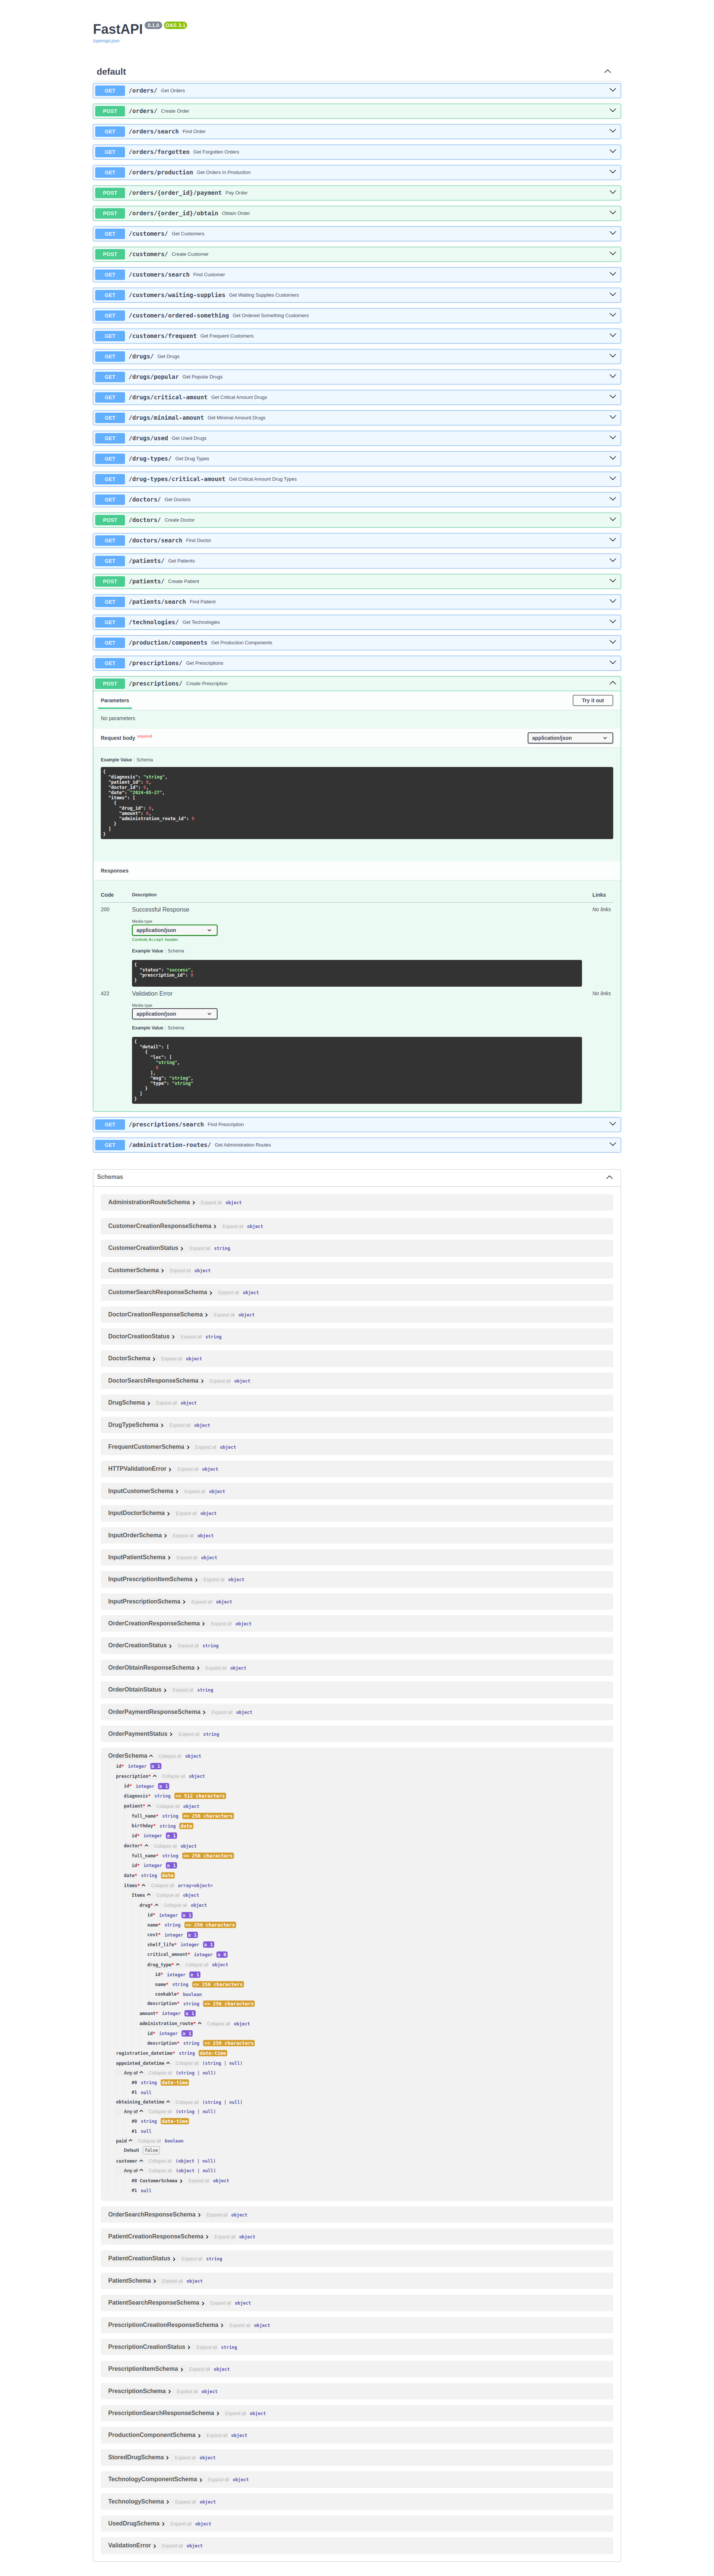
\includegraphics[scale=0.1]{screens/openapi}
				\caption{Документация к веб-серверу в формате OpenAPI}
			\end{figure}
			
		\subsection{Клиентская часть}
			Клиентская часть включает в себя:
			\begin{itemize}
				\item desktop-приложение для работников кассы аптеки;
				
				\item панель администратора для системных администраторов.
			\end{itemize}

			\subsubsection{Desktop-приложение}
				Desktop-приложение написано на языке программирования Java-17 с использованием платформы Swing. Приложение позволяет:
				\begin{itemize}
					\item просматривать содержимое некоторых (нужных для работников кассы) таблиц;
					
					\item выполнять все запросы к информационной системе;
					
					\item создавать и изменять заказы посетителей аптеки.
				\end{itemize}
					
				\begin{figure}[H]
					\centering
					\fbox{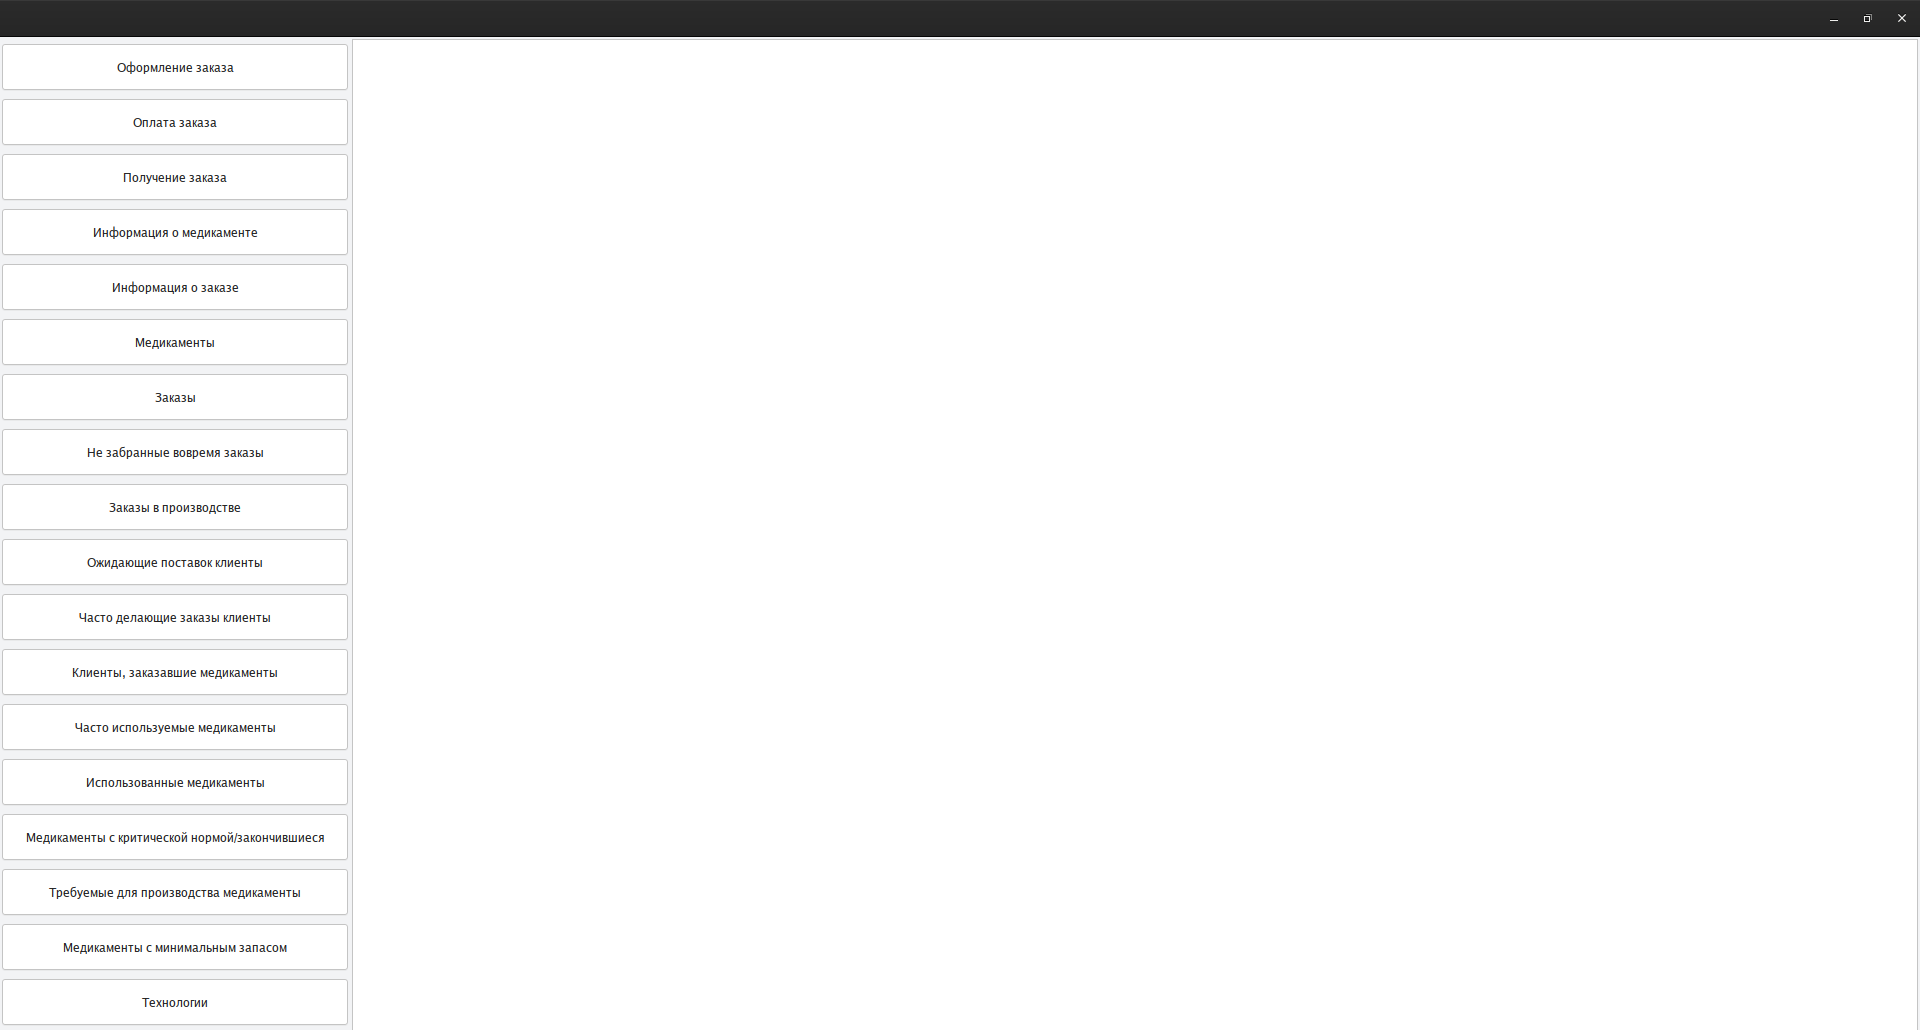
\includegraphics[scale=0.25]{screens/desktop}}
					\caption{Окно приложения}
				\end{figure}
				
				\begin{figure}[H]
					\centering
					\fbox{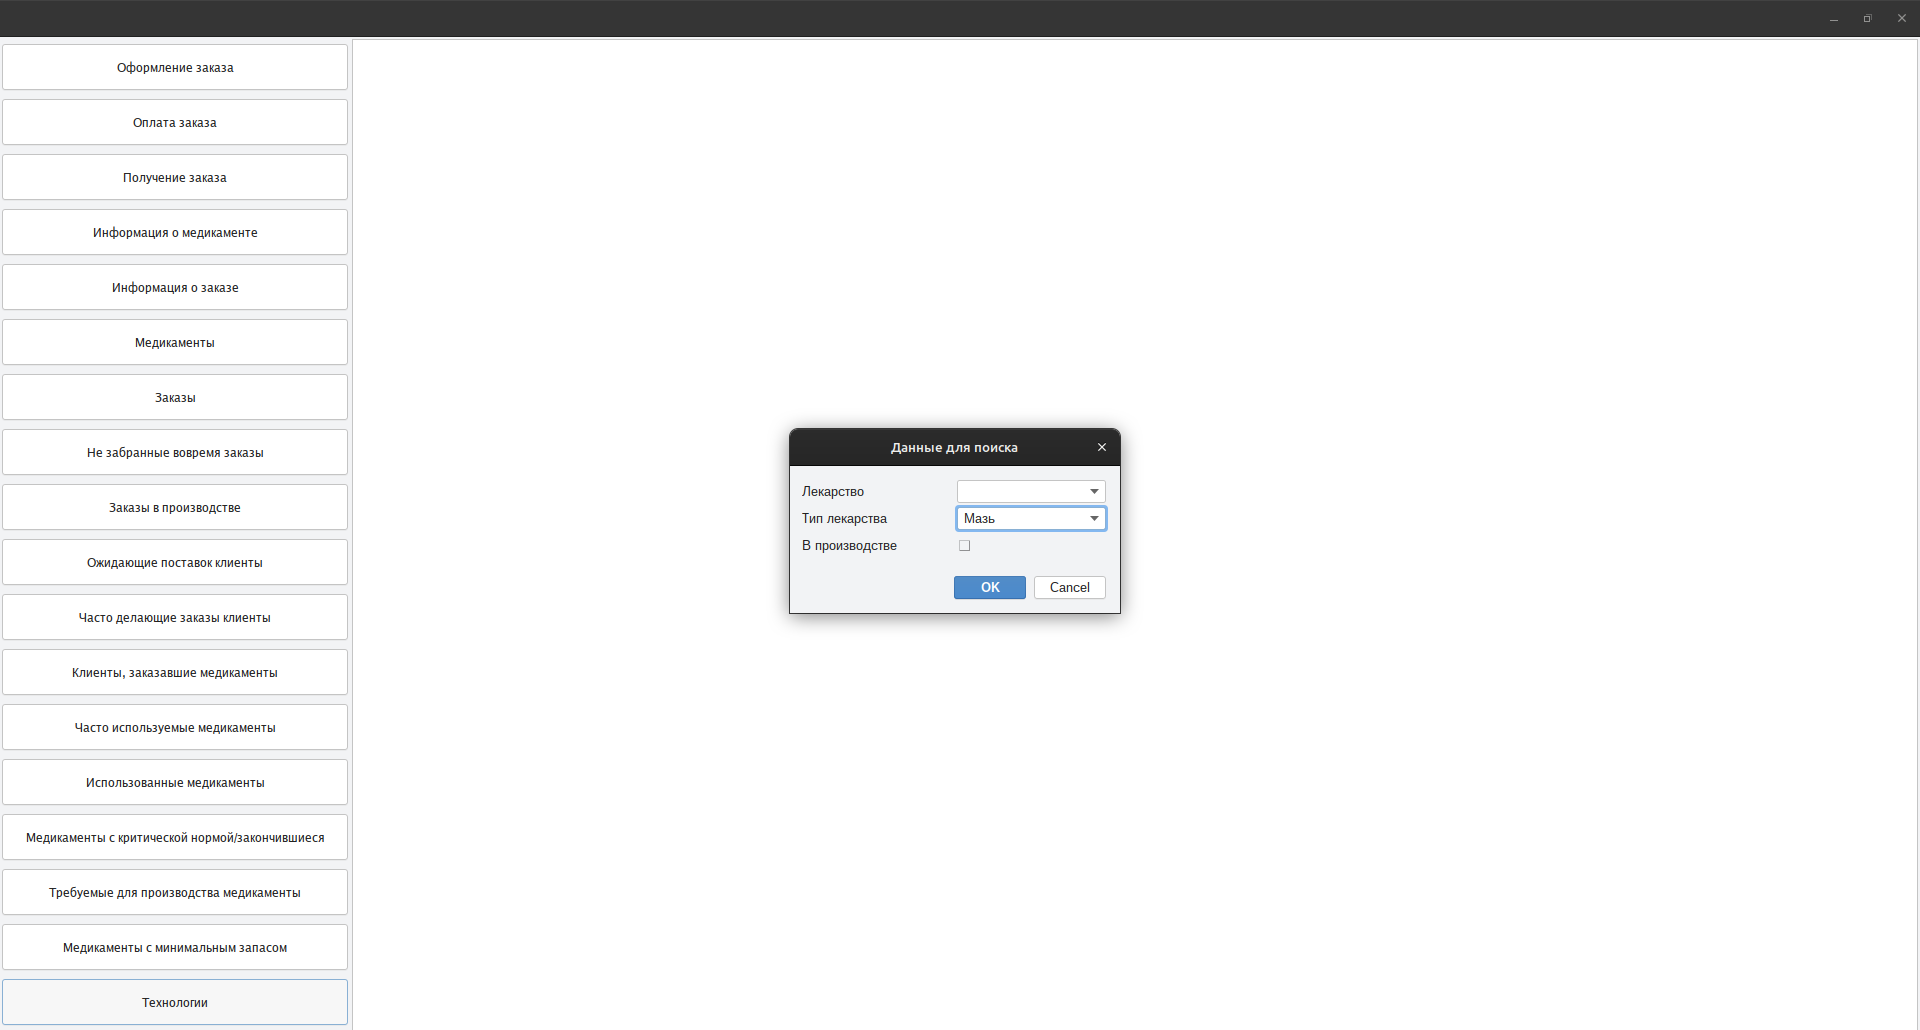
\includegraphics[scale=0.25]{screens/desktop-modal-window}}
					\caption{Пример модального окна для ввода параметров запроса}
				\end{figure}
			
				\begin{figure}[H]
					\centering
					\fbox{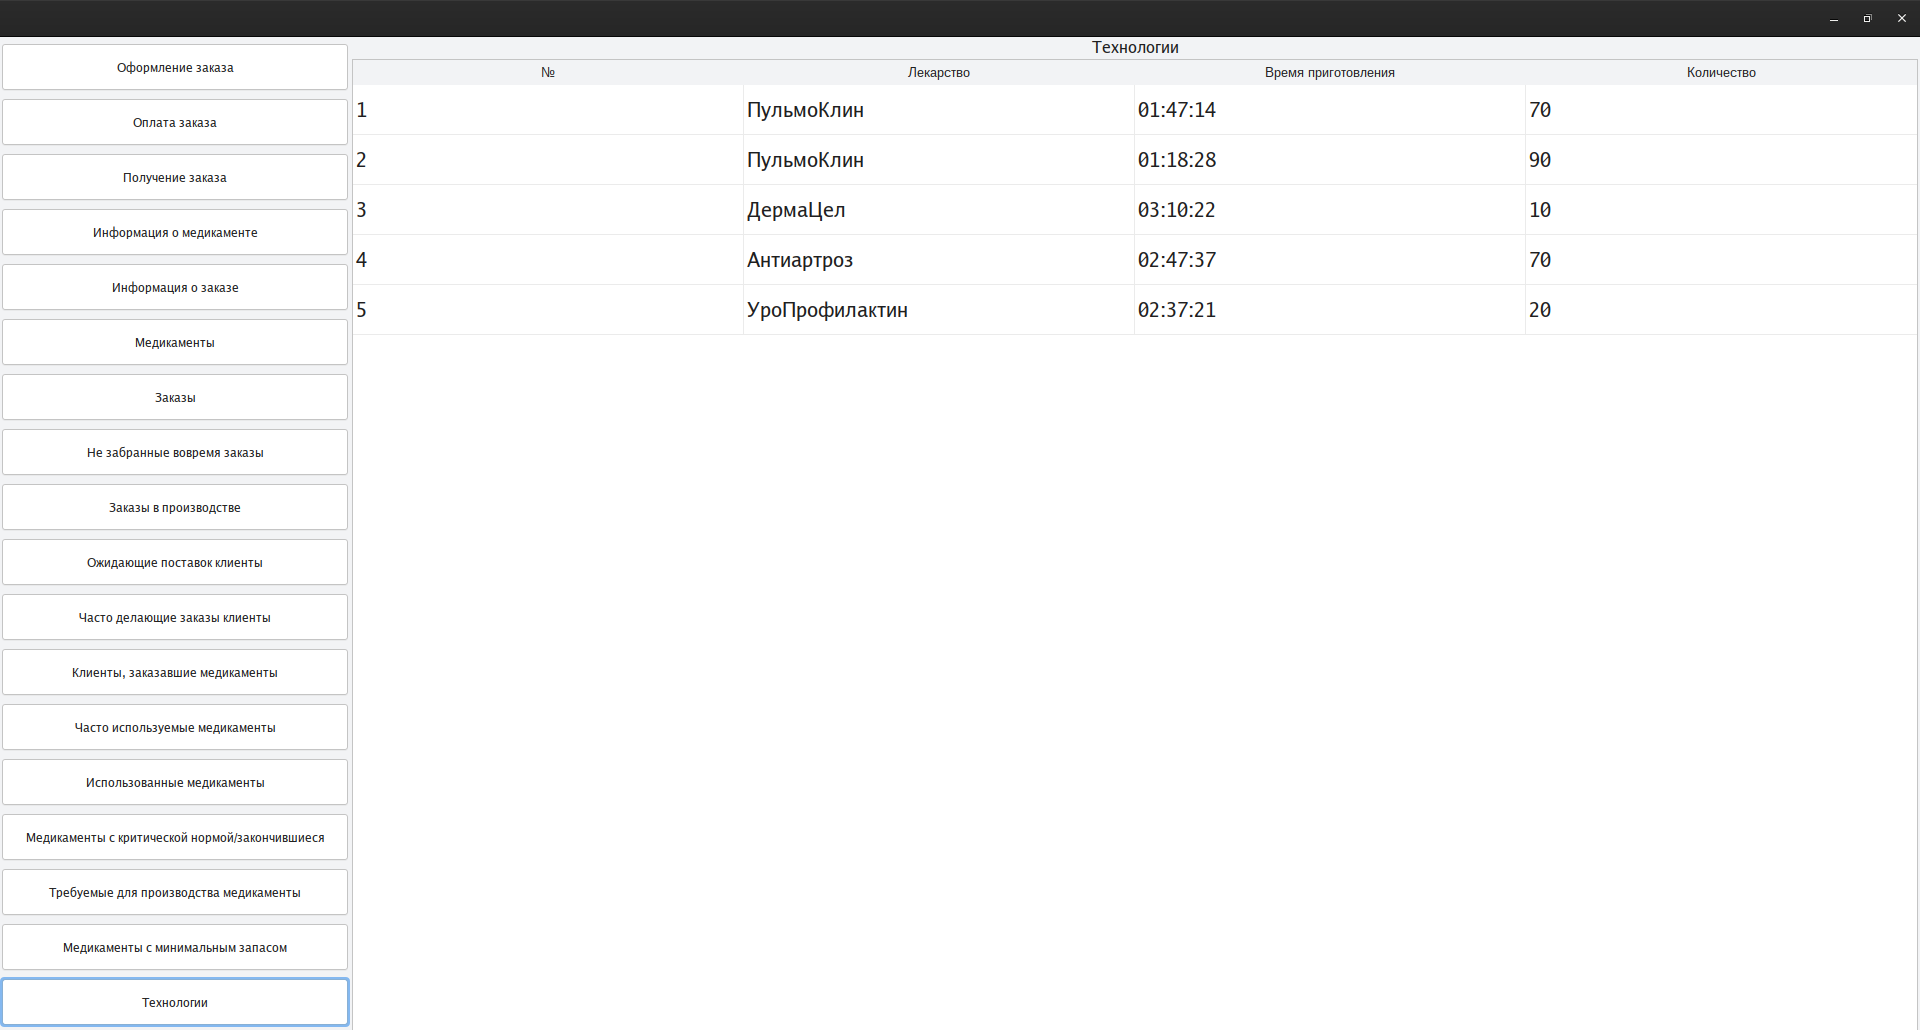
\includegraphics[scale=0.25]{screens/desktop-table}}
					\caption{Пример результата выполнения запроса}
				\end{figure}
			
				\begin{figure}[H]
					\centering
					\fbox{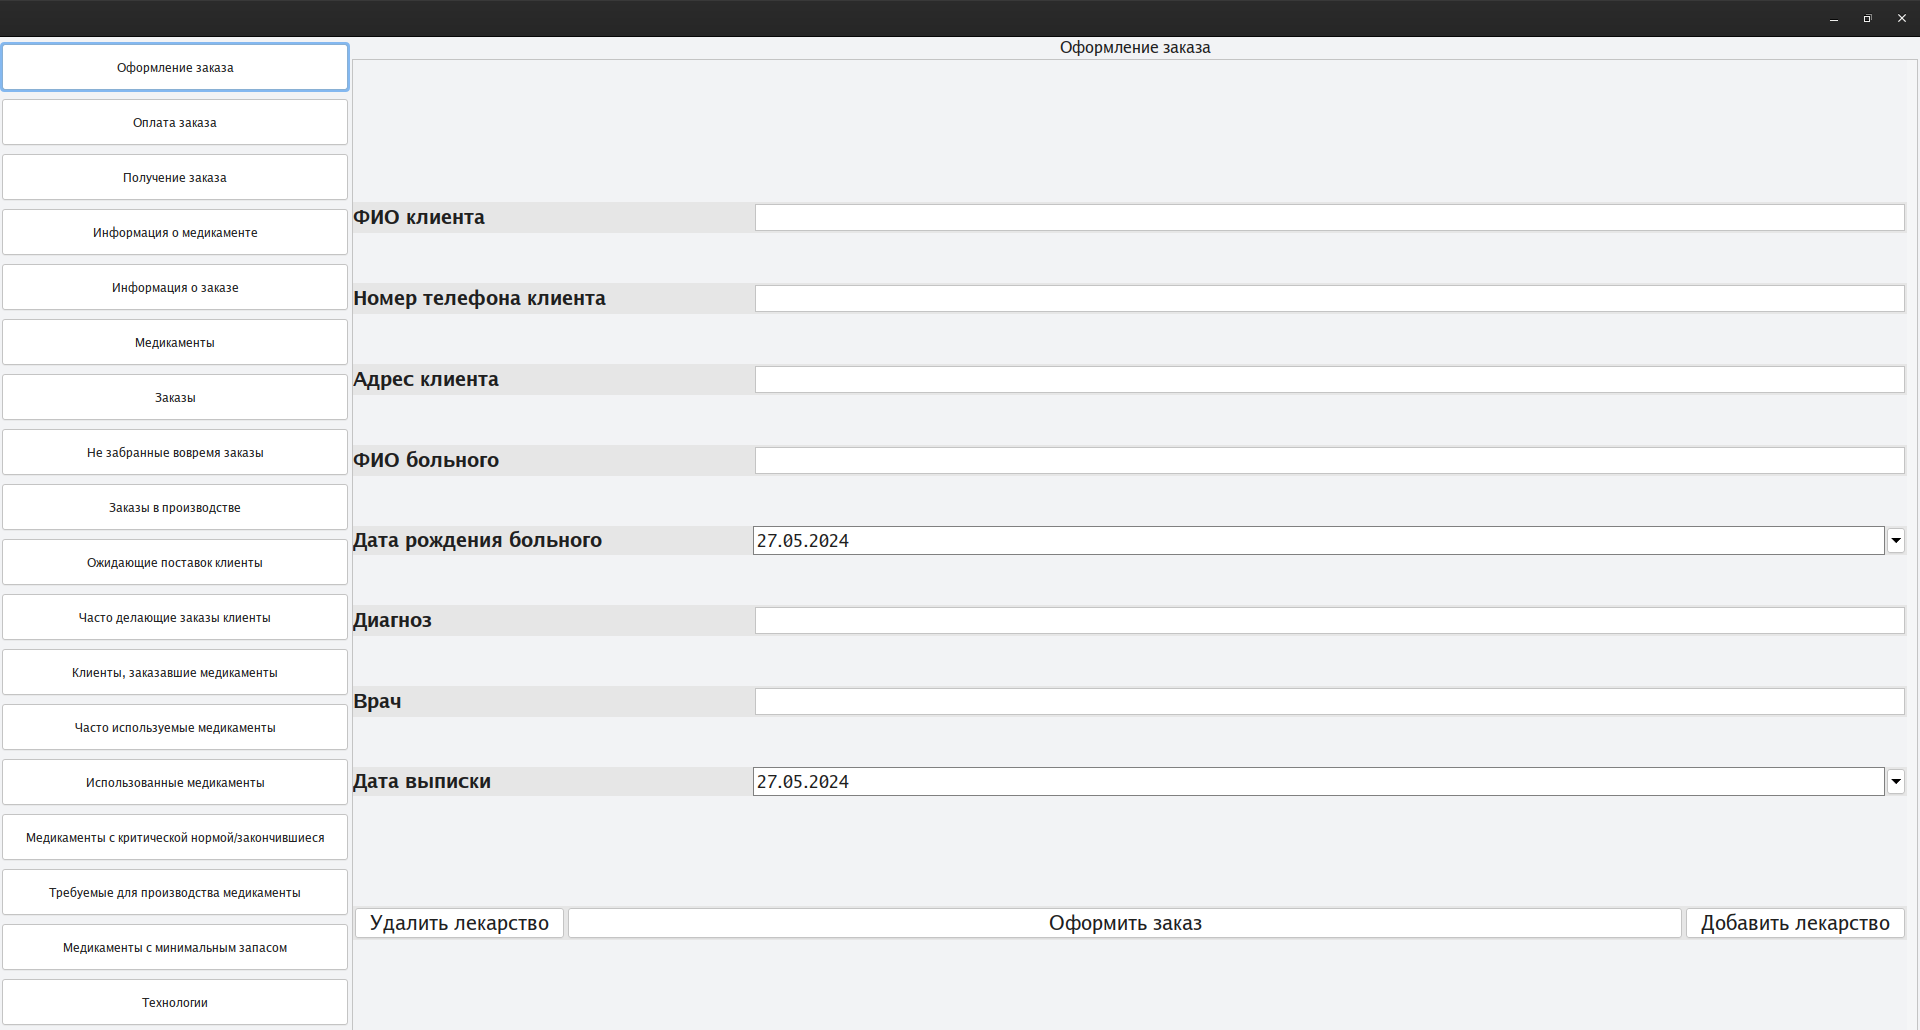
\includegraphics[scale=0.25]{screens/desktop-order-creation}}
					\caption{Форма для оформления заказа}
				\end{figure}

				\begin{figure}[H]
					\centering
					\fbox{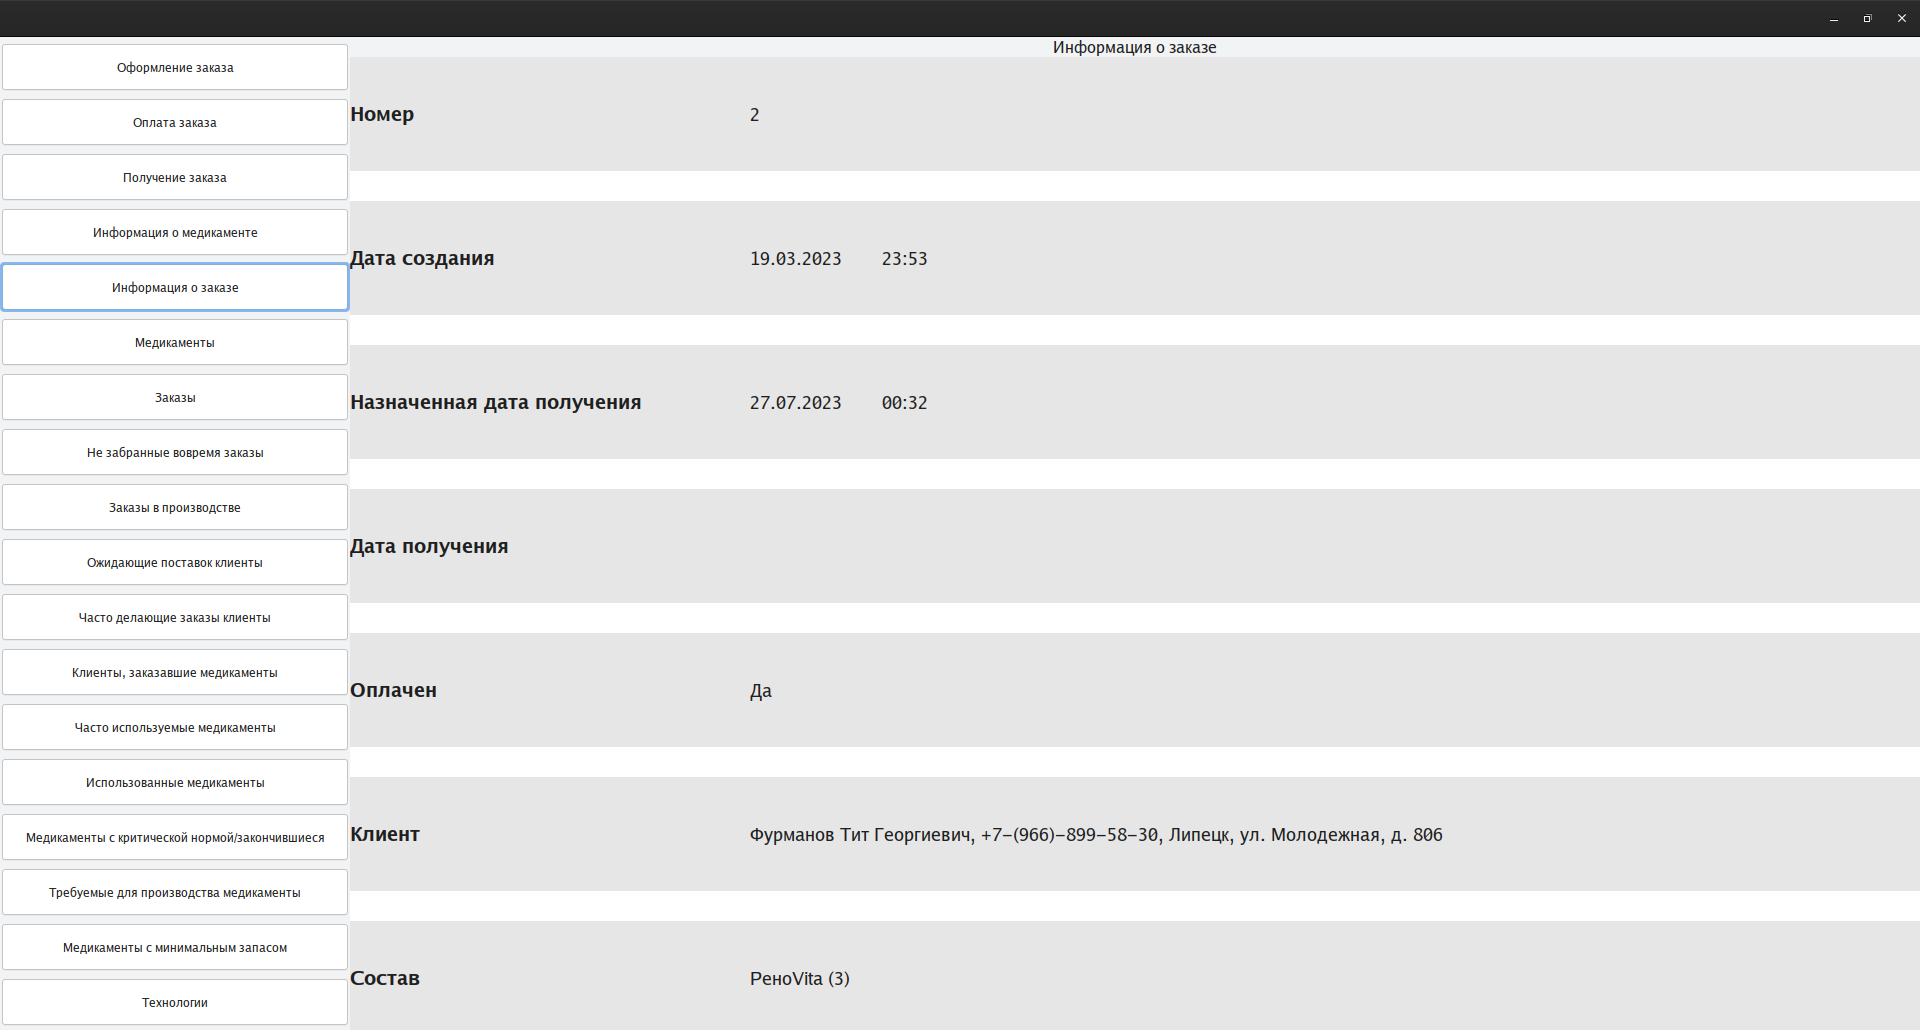
\includegraphics[scale=0.25]{screens/desktop-order-info}}
					\caption{Панель с информацией о заказе}
				\end{figure}

				\begin{figure}[H]
					\centering
					\fbox{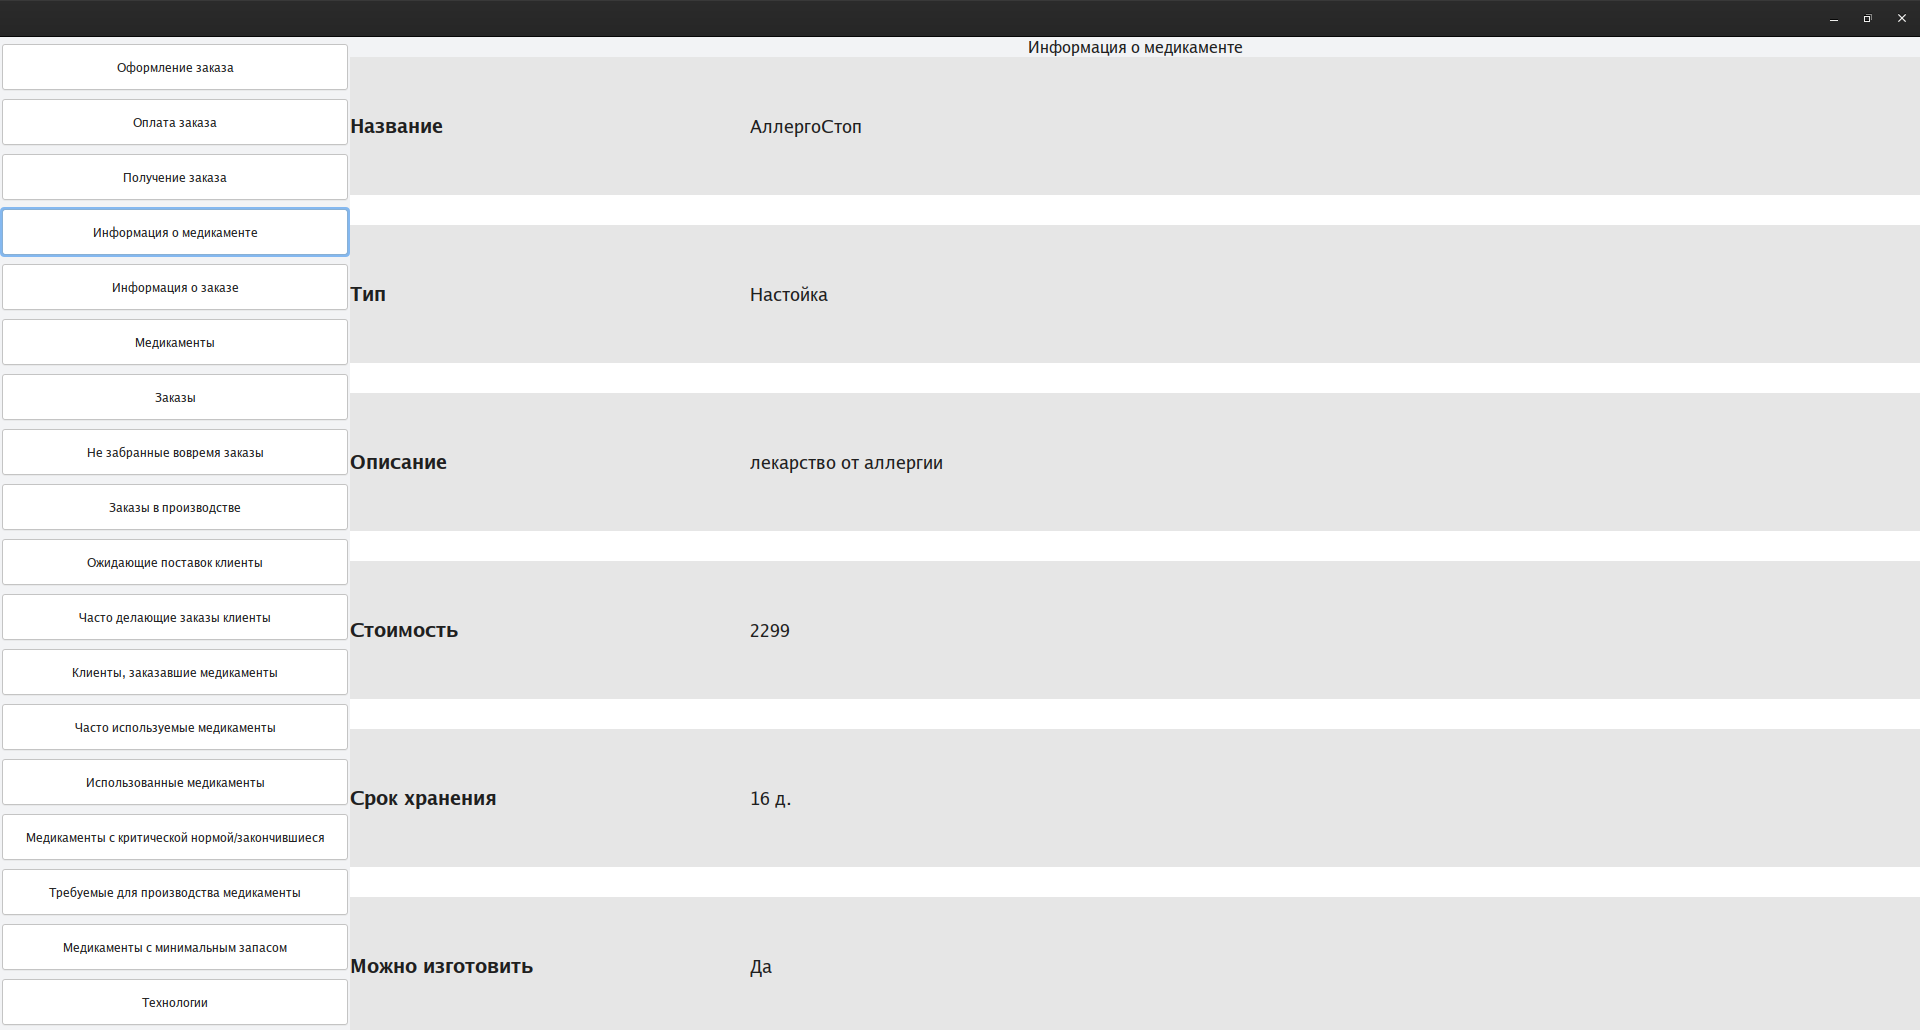
\includegraphics[scale=0.25]{screens/desktop-drug-info}}
					\caption{Панель с информацией о медикаменте}
				\end{figure}
				
				\begin{figure}[H]
					\centering
					\fbox{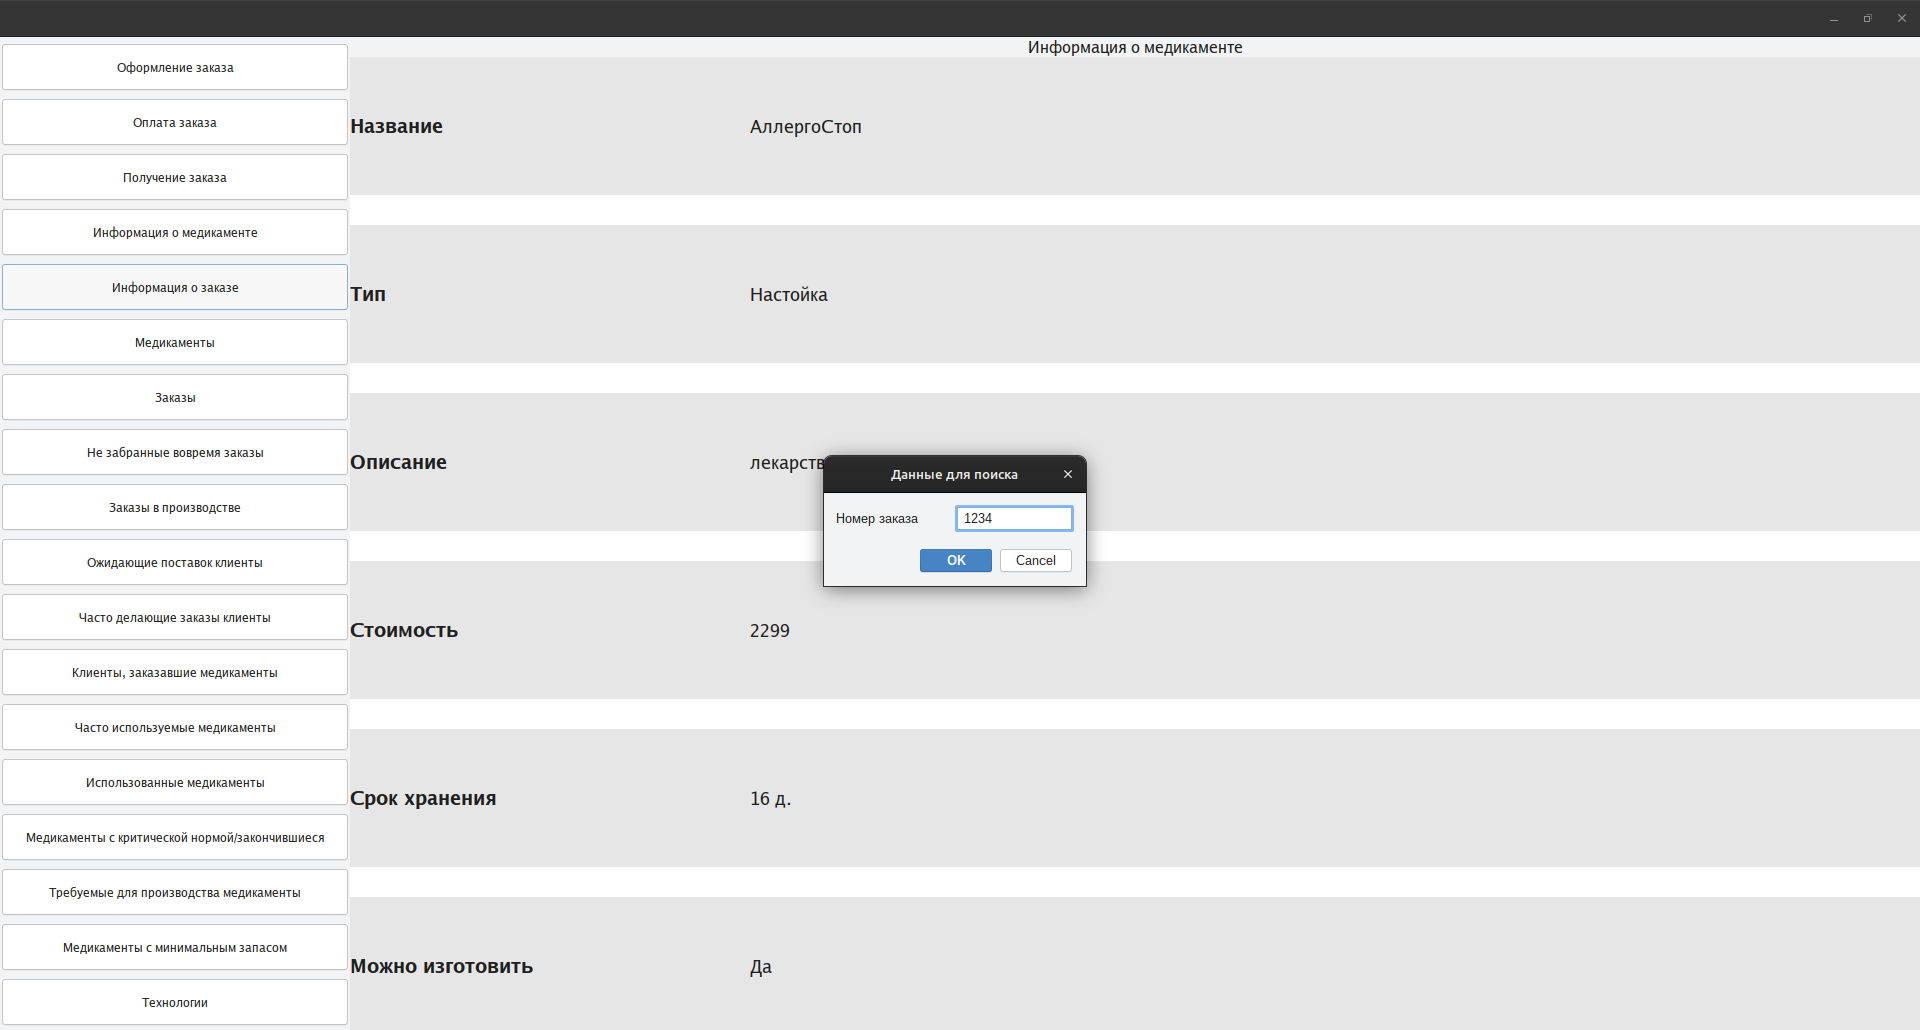
\includegraphics[scale=0.25]{screens/desktop-order-info-model-window}}
					\caption{Модальное окно для ввода номера заказа, по которому будет осуществлён поиск информации}
				\end{figure}
				
				\begin{figure}[H]
					\centering
					\fbox{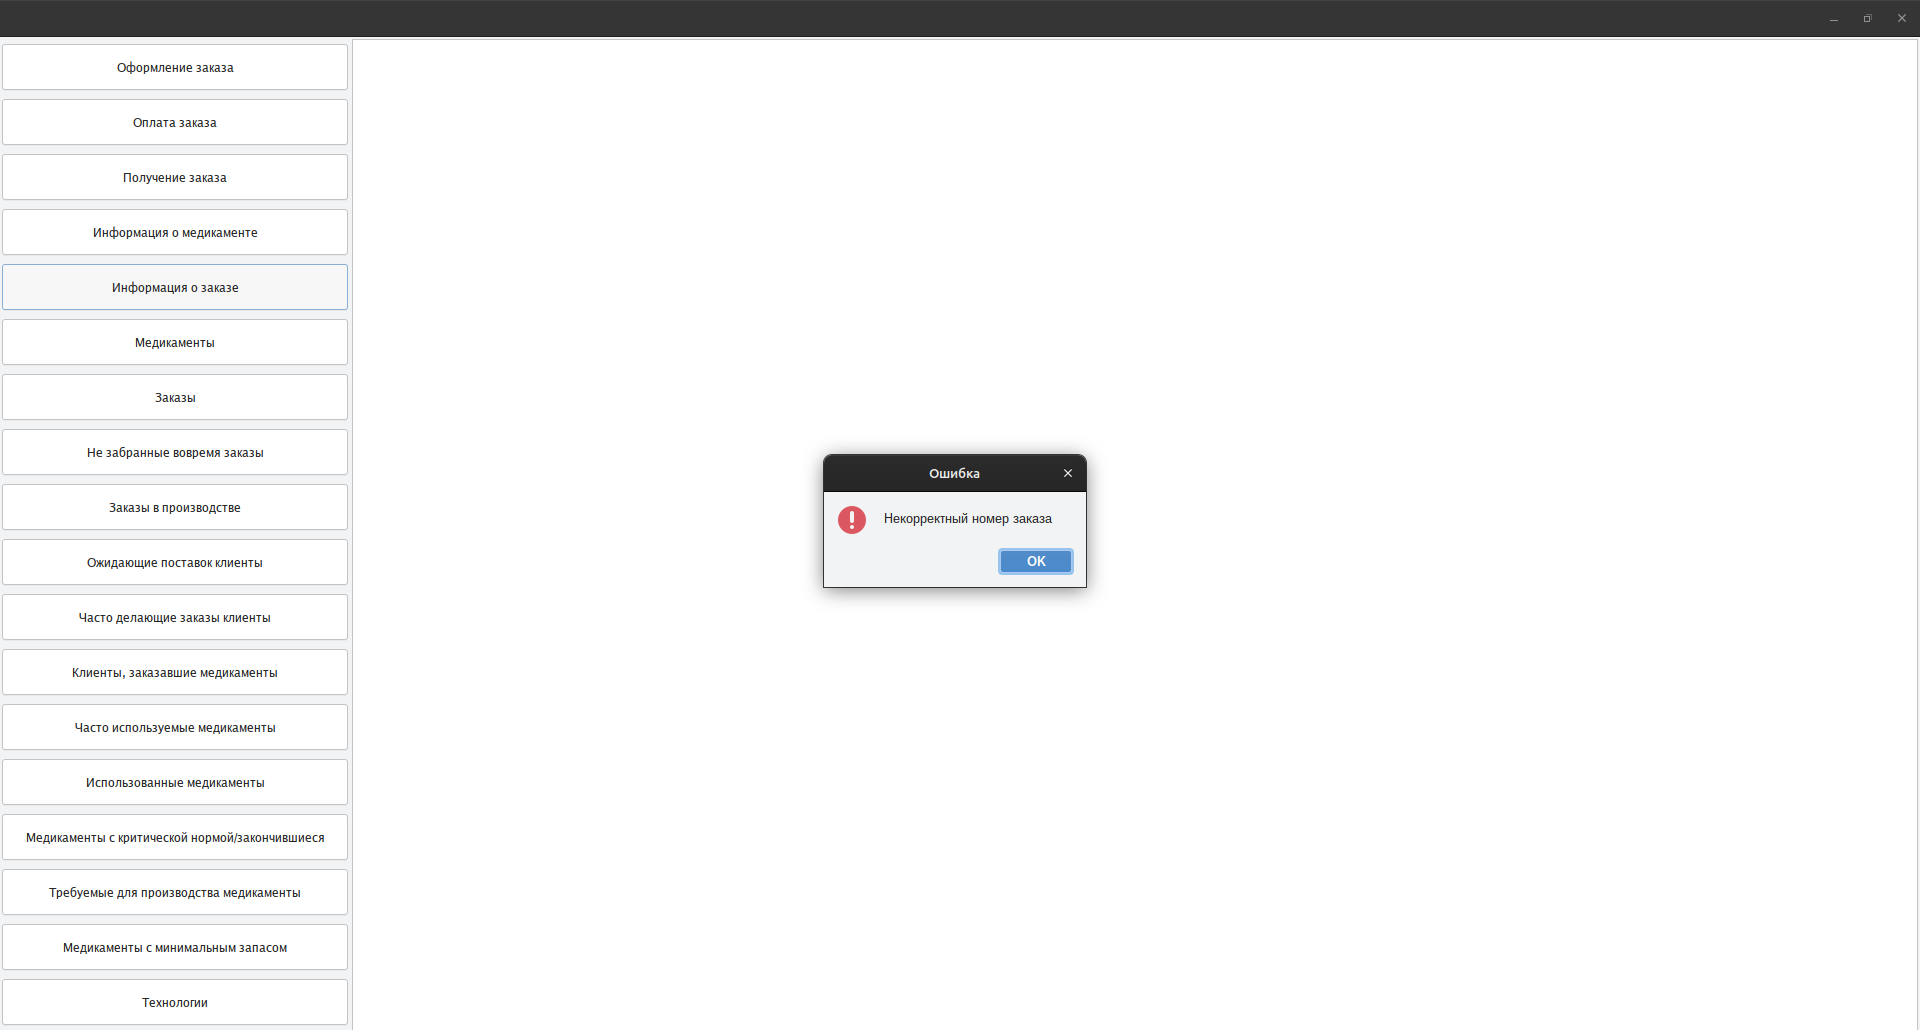
\includegraphics[scale=0.25]{screens/desktop-invalid-order-message}}
					\caption{Сообщение о некорректном номере заказа}
				\end{figure}
				
				\begin{figure}[H]
					\centering
					\fbox{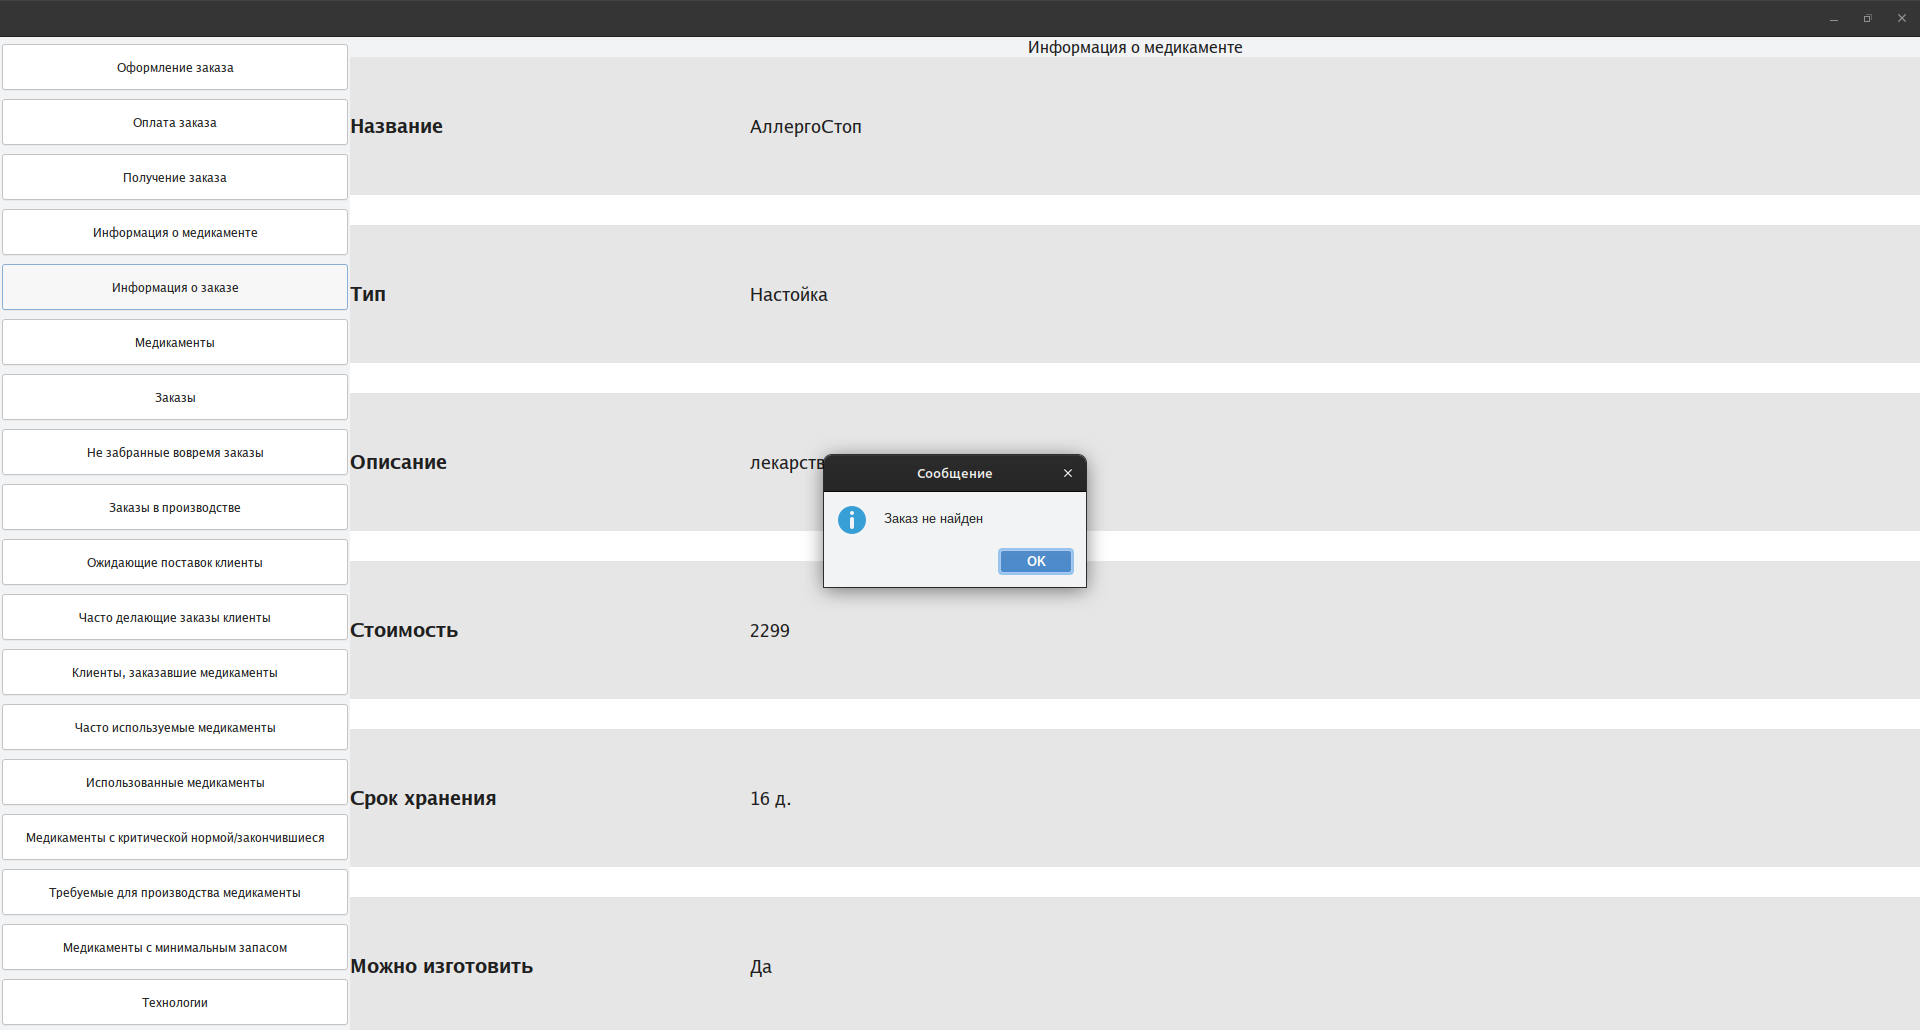
\includegraphics[scale=0.25]{screens/desktop-order-not-found-message}}
					\caption{Сообщение о том, что заказ не найден}
				\end{figure}
			\subsubsection{Панель администратора}
				Панель администратора представляет собой сайт, запущенный на том же веб-сервере, что и серверная часть. Панель администратора позволяет просматривать, изменять и удалять содержимое всех таблиц.
				
				\begin{figure}[H]
					\centering
					\fbox{
\includegraphics[scale=0.25]{screens/admin-panel}}
					\caption{Общий вид панели администратора}
				\end{figure}
				
				\begin{figure}[H]
					\centering
					\fbox{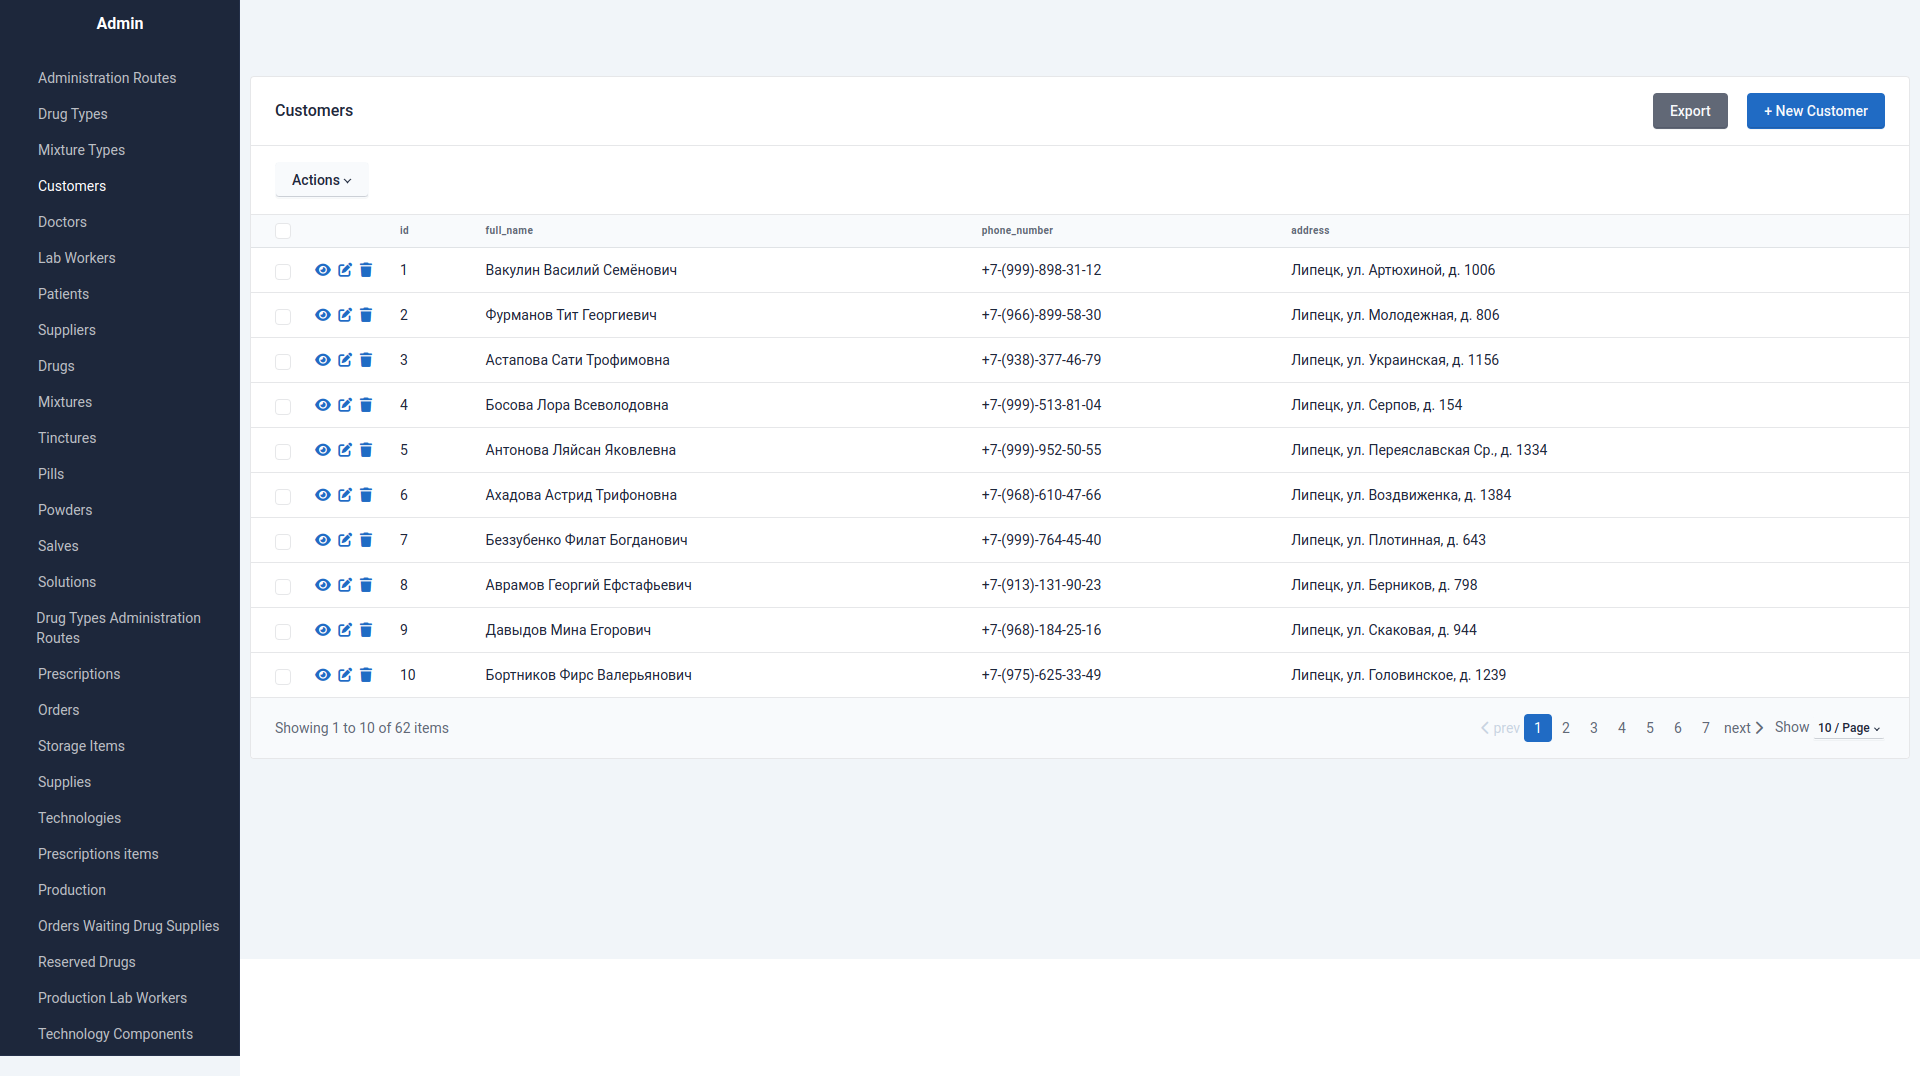
\includegraphics[scale=0.25]{screens/admin-panel-table}}
					\caption{Пример просмотра содержимого таблицы}
				\end{figure}
				
				\begin{figure}[H]
					\centering
					\fbox{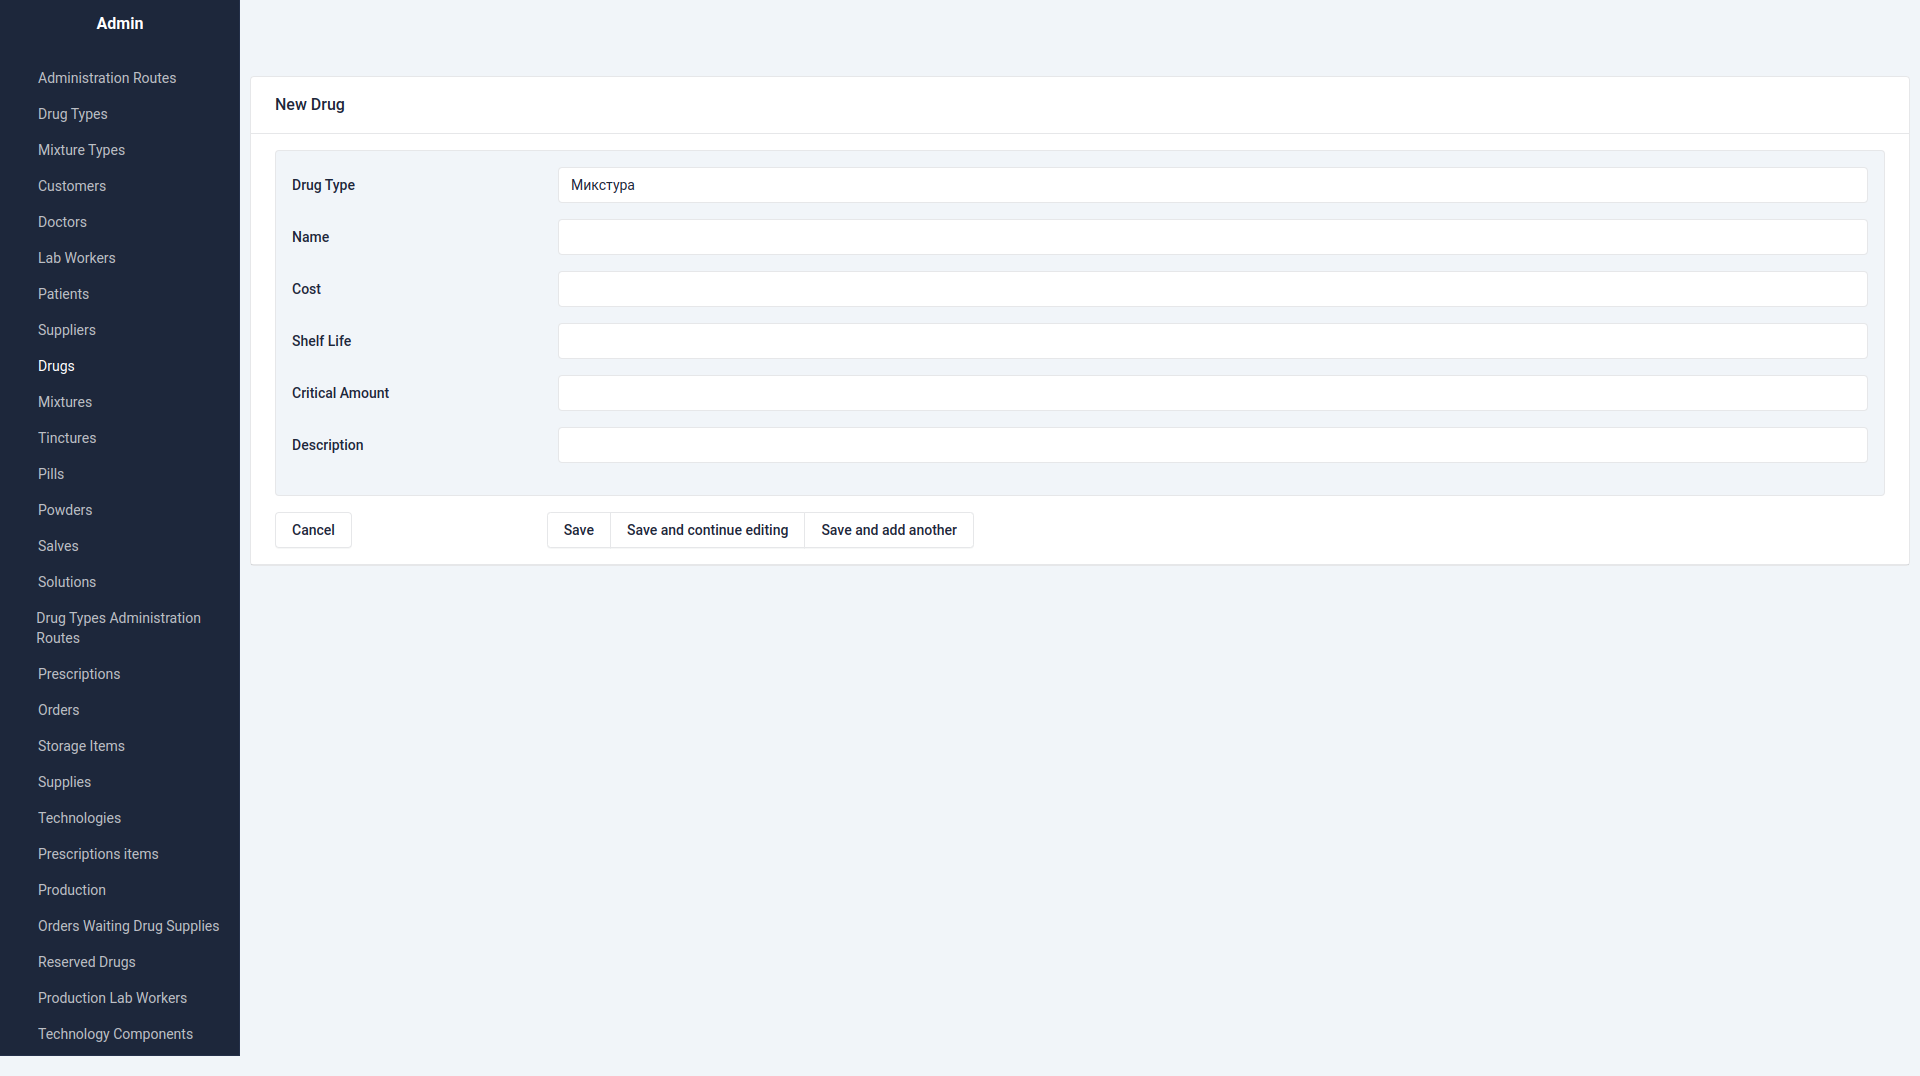
\includegraphics[scale=0.25]{screens/admin-panel-new}}
					\caption{Пример формы для добавления записи в таблицу}
				\end{figure}
				
				\begin{figure}[H]
					\centering
					\fbox{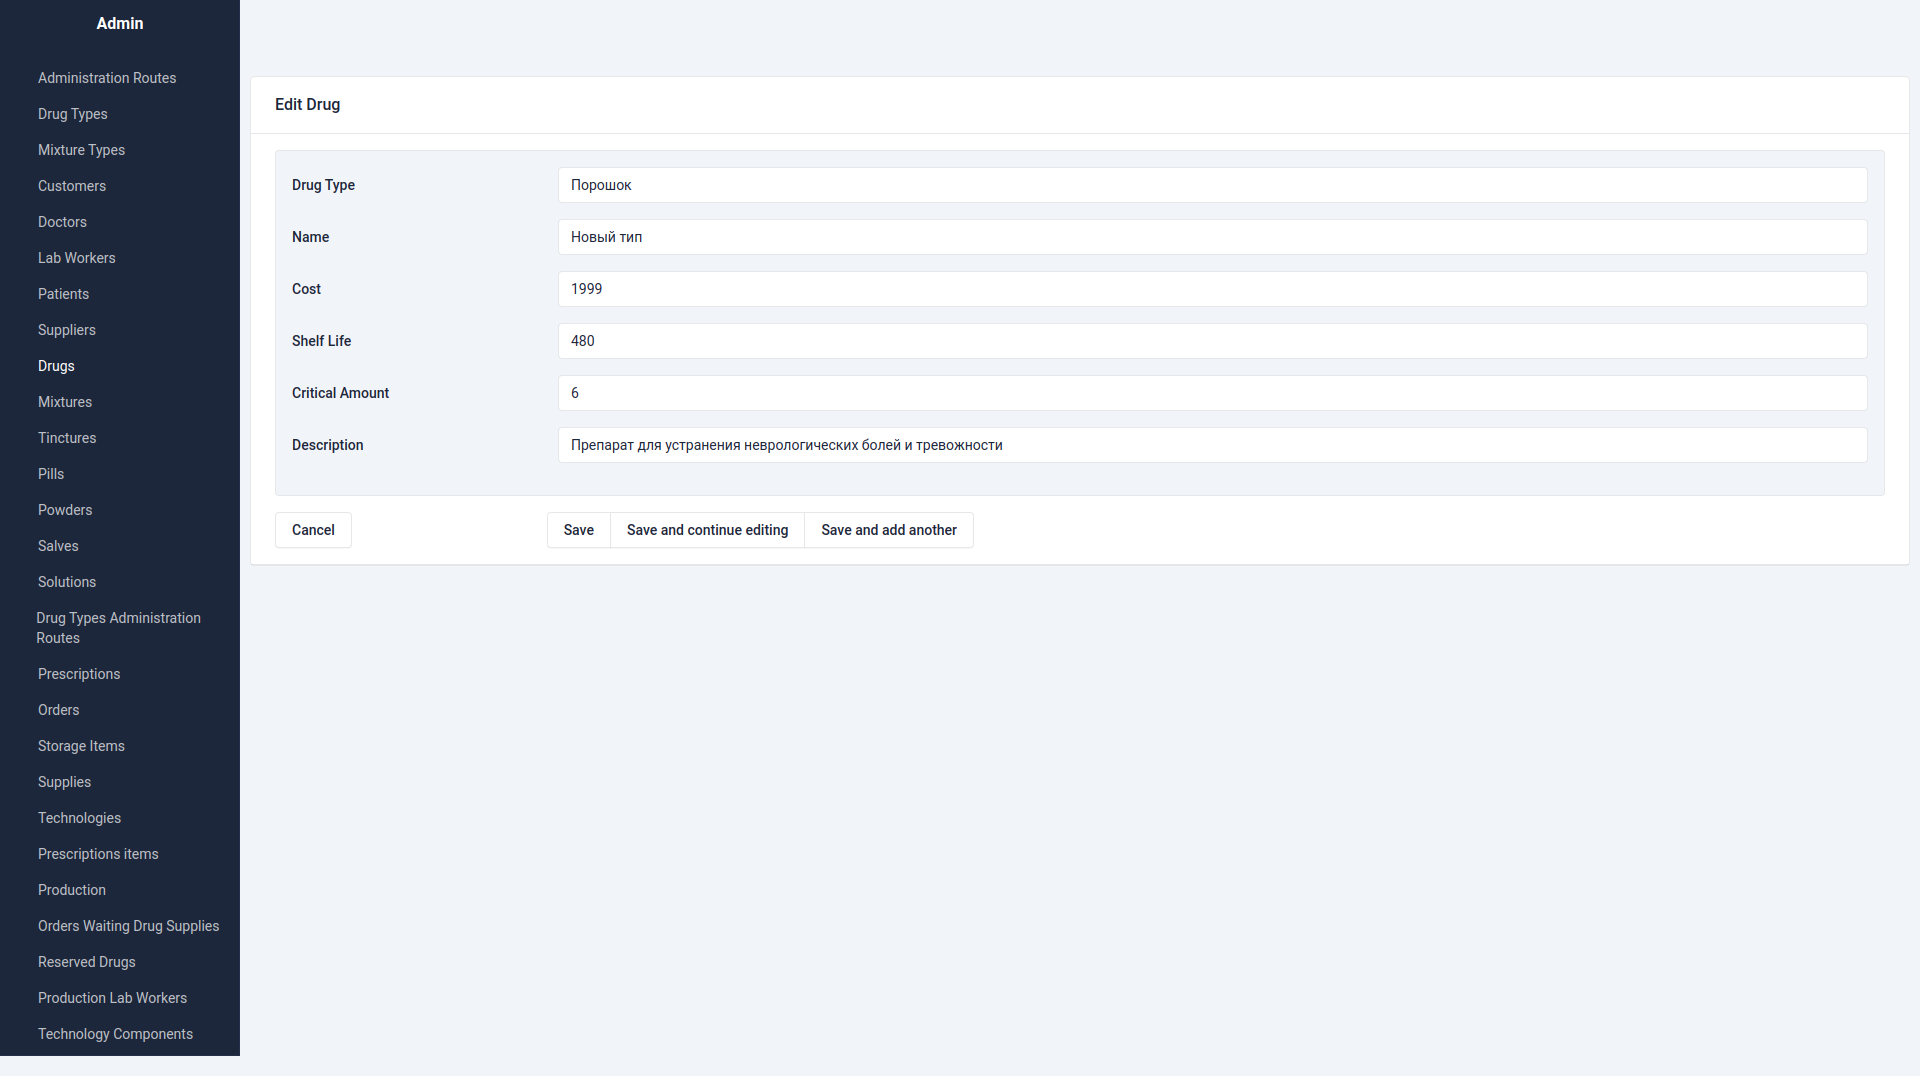
\includegraphics[scale=0.25]{screens/admin-panel-edit}}
					\caption{Пример формы для изменения записи таблицы}
				\end{figure}
				
				\begin{figure}[H]
					\centering
					\fbox{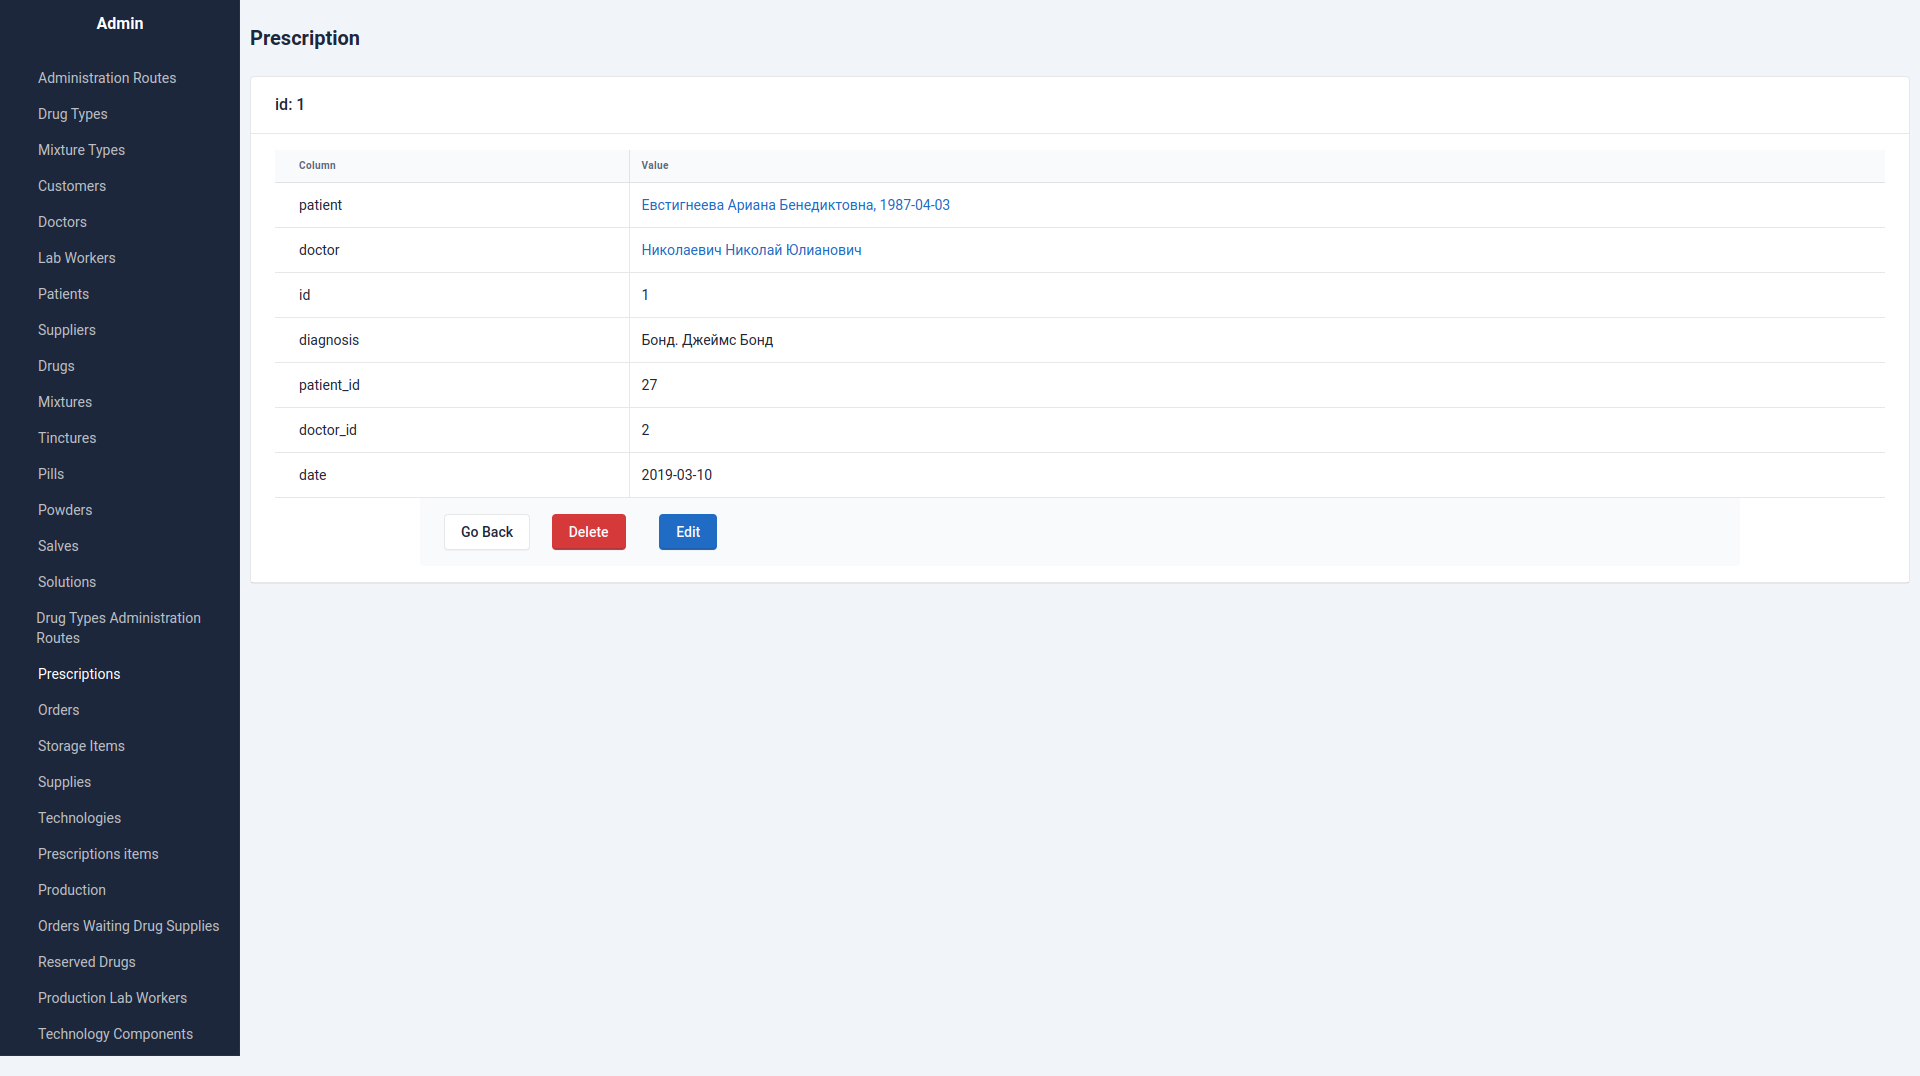
\includegraphics[scale=0.25]{screens/admin-panel-info}}
					\caption{Пример просмотра подробной информации о записи таблицы}
				\end{figure}
		
	\newpage
				
	\section{Выводы}
		В ходе работы была разработана структура базы данных информационной системы аптеки, а также реализованы серверная и клиентская части системы. выполняющие операции внесения данных в базу данных, редактирование данных и запросы.
\end{document}
